\documentclass%
%[handout]
{beamer}
% % % % % % % %
% % % % % % % %
% % % % % % % %
%IMPORTANT
%compiles with 
%pdflatex -shell-escape 
%IMPORTANT
% % % % % % % %
% % % % % % % %
% % % % % % % %
\mode<presentation>
{
\useinnertheme{rounded}
\useoutertheme{infolines}
\usecolortheme{orchid}
\usecolortheme{whale}
}

\usepackage[english]{babel}
\usepackage[latin1]{inputenc}
\usepackage[all,cmtip]{xy}
\usepackage{times}
\usepackage[T1]{fontenc}
\usepackage{../example-templates}
\usepackage{../pstricks-commands}

\usepackage{auto-pst-pdf}
\usepackage{pst-plot}
%\usepackage{pstricks-add} 

% Or whatever. Note that the encoding and the font should match. If T1
% does not look nice, try deleting the line with the fontenc.


\graphicspath{{../../modules/}}

\newtheoremstyle{partialproof}{3pt}{3pt}{}{}{}{.}{.5em}{}
\theoremstyle{partialproof} \newtheorem{partialproof}[theorem]{Proof.}
%\DeclareMathOperator{\diff}{d}
\setbeamertemplate{navigation symbols}{}

\includeonlylecture{1}

\newcommand{\lect}[3]{
  \date{#1}
  \lecture[#1]{#2}{#3}
}

\setbeamertemplate{footline}
{
  \leavevmode%
  \hbox{%
  \begin{beamercolorbox}[wd=.333333\paperwidth,ht=2.25ex,dp=1ex,center]{author in head/foot}%
    \usebeamerfont{author in head/foot}\insertshortauthor
  \end{beamercolorbox}%
  \begin{beamercolorbox}[wd=.333333\paperwidth,ht=2.25ex,dp=1ex,center]{title in head/foot}%
    \usebeamerfont{title in head/foot}\insertshorttitle
  \end{beamercolorbox}%
  \begin{beamercolorbox}[wd=.333333\paperwidth,ht=2.25ex,dp=1ex,center]{date in head/foot}%
    \usebeamerfont{date in head/foot}\insertshortdate{}
  \end{beamercolorbox}}%
  \vskip0pt%
}

% If you have a file called "university-logo-filename.xxx", where xxx
% is a graphic format that can be processed by latex or pdflatex,
% resp., then you can add a logo as follows:

%\pgfdeclareimage[height=0.8cm]{logo}{bluelogo}
%\logo{\pgfuseimage{logo}}
\renewcommand{\Arcsin}{\arcsin}
\renewcommand{\Arccos}{\arccos}
\renewcommand{\Arccot}{\text{arccot}}
\renewcommand{\Arctan}{\arctan}


\begin{document}

\AtBeginLecture{%

\title[\insertlecture]{FreeCalc}
\subtitle{\insertlecture}
\author[FreeCalc]{}
\institute[UMass Boston]{University of Massachusetts Boston}
\date{\insertshortlecture}
\begin{frame}
  \titlepage
\end{frame}
}%

% begin lecture
\lect{\today}{Sample}{1}

\begin{frame}
\frametitle{Geometric interpretation of all trigonometric functions}
\vskip -0.1cm
\begin{columns}
\column{0.35\textwidth}
\psset{xunit=1.5cm,yunit=1.5cm}
\begin{pspicture}(-1.3,-1.3)(1.3,2.5)
\tiny
\rput[rb](-0.1,1){$1$}
%circle:
\pstVerb{20 dict begin 
/theta 65 def
/sintheta theta sin def
/costheta theta cos def
/tantheta theta sin theta cos div def
/cottheta 1 tantheta div def
/csctheta 1 sintheta div def
/sectheta 1 costheta div def
/heelSize 0.09 def
/angleRadius 0.25 def
}
\parametricplot[linecolor=\fcColorGraph, plotpoints=500]{0}{360}{t cos t sin}
\psline(1, -1.3)(1,2.5)

\uncover<2->{
\psline(0,0)(! 1 tantheta)
}
%angle:
\psaxes[ticks=none, labels=none]{<->}(0,0)(-1.2,-1.2)(1.2,1.2)

\uncover<2->{
\rput[lb](0.22, 0.16){$\alertNoH{2,6,23,11,12,17,18,30,41,47,48,53,59}{\theta}$}
\parametricplot[plotpoints=200]{0}{theta}{t cos angleRadius mul t sin angleRadius mul}
\rput[l](! 1.05 tantheta){\alertNoH{2}{$B$}}
\rput[bl](1.05,0.05){\alertNoH{2}{$D$}}
}
\uncover<handout:0|6,11,12,17,18,23,30,41,47,48,53,59>{
\parametricplot[plotpoints=200, linecolor=red, linewidth=2pt]{0}{theta}{t cos angleRadius mul t sin angleRadius mul}
}
\psline(! 1 heelSize sub 0)(! 1 heelSize sub heelSize)(! 1 heelSize)
\uncover<handout:0|29>{
\psline[plotpoints=200, linecolor=red, linewidth=2pt](! 1 heelSize sub 0)(! 1 heelSize sub heelSize)(! 1 heelSize)
}

\rput[tr](-0.1,-0.1){\alertNoH{2}{$O$}}
\uncover<3->{
\rput[b](0.4,1){\alertNoH{3}{$A$}}
}
\uncover<5->{
\psline[linecolor=black](! costheta sintheta)(! costheta 0)
\rput[tl](! costheta -0.05){$C$}
\psline(! costheta heelSize sub 0)(! costheta heelSize sub heelSize)(! costheta heelSize)
}
\uncover<9->{
\rput[b](! costheta 0.5 mul sintheta 0.5 mul 0.1 add){$\alertNoH{9,15}{1}$}
}
\uncover<11->{
\psline[linecolor=blue, linewidth=1.05pt](! costheta sintheta)(! costheta 0)
}
\uncover<17->{
\psline[linecolor=green, linewidth=1.05pt](0,0)(! costheta 0)
}
\uncover<23->{%
\psline[linecolor=purple, linewidth=1.05pt](1,0)(! 1 tantheta)%
}%
\uncover<handout:0|23>{%
\psline[linecolor=purple, linewidth=2.4pt](1,0)(! 1 tantheta)%
}%
\uncover<25->{%
\psline(! sintheta heelSize mul costheta -1 mul heelSize mul)(! sintheta heelSize mul costheta heelSize mul add costheta -1 mul heelSize mul sintheta heelSize mul add) (! costheta heelSize mul sintheta heelSize mul)%
\rput[l](1.05,-0.5){$E$}%
\psline[linecolor=black](0,0)(! 1 cottheta -1 mul)%
%\fcAngle{90}{90 2 atan add}{0.2}{$\theta$}
}%

\uncover<handout:0|25>{
\psline[linecolor=red, linewidth=2pt](0,0)(! 1 cottheta -1 mul)%
}
\uncover<26->{
\parametricplot[plotpoints=200]{90}{theta 90 add}{t cos angleRadius mul 1 add t sin angleRadius mul theta cos theta sin div sub}
}
\uncover<26->{
\rput[rb](0.9,-0.2){$\alertNoH{26,33,34,42,54}{\fcAnswerUncover{26}{41}{\theta}} $}%
}
\uncover<handout:0|26,33,34,40,41,42,54>{
\parametricplot[plotpoints=200, linecolor=red, linewidth=2pt]{90}{theta 90 add}{t cos angleRadius mul 1 add t sin angleRadius mul cottheta sub}
}
\uncover<27->{
\parametricplot[plotpoints=200]{-90}{-180 theta add}{t cos angleRadius mul 1 add t sin angleRadius mul tantheta add}
\rput[tl](! 0.85 tantheta -0.3 add ){$\alertNoH{27,28,32,36}{\beta}$}
}
\uncover<handout:0|27,28,32,36>{
\parametricplot[plotpoints=200, linecolor=red, linewidth=2pt]{-90}{-180 theta add}{t cos angleRadius mul 1 add t sin angleRadius mul tantheta add}
}
\uncover<handout:0|25,35>{
\psline[linewidth=2pt, linecolor=red](! sintheta heelSize mul costheta -1 mul heelSize mul)(! sintheta heelSize mul costheta heelSize mul add costheta -1 mul heelSize mul sintheta heelSize mul add) (! costheta heelSize mul sintheta heelSize mul)%
}
\uncover<53->{%
\psline[linecolor=magenta, linewidth=1.05pt](0,0)(! 1 tantheta)%
}%
\uncover<handout:0|53>{
\psline[linecolor=magenta, linewidth=2.4pt](0,0)(! 1 tantheta)
}
\uncover<handout:0|25>{%
\psline[linecolor=magenta, linewidth=2pt](0,0)(! 1 tantheta)%
}%
\uncover<32->{
\psline[linecolor=black](0,0)(! 1 cottheta -1 mul)
}
\uncover<59->{
\psline[linecolor=brown, linewidth=1.05pt](0,0)(! 1 cottheta -1 mul)
}
\uncover<handout:0|59>{
\psline[linecolor=brown, linewidth=2.4pt](0,0)(! 1 cottheta -1 mul)
}
\uncover<47->{%
\psline[linecolor=cyan, linewidth=1.05pt](1,0)(! 1 cottheta -1 mul)%
}%
\uncover<handout:0|47>{%
\psline[linecolor=cyan, linewidth=2.4pt](1,0)(! 1 cottheta -1 mul)%
}%
\uncover<handout:0|6-10,12-16>{
\psline[linecolor=red, linewidth=2pt](0,0)(! costheta 0)(! costheta sintheta)(0,0)(! costheta 0)
}
\uncover<handout:0|13,14-17>{
\psline[linecolor=green, linewidth=2pt](0,0)(! costheta 0)
}
\uncover<handout:0|7,8-11>{
\psline[linecolor=blue, linewidth=2pt](! costheta sintheta)(! costheta 0)
}
\uncover<handout:0|8-10,14-16>{%
\psline[linecolor=orange, linewidth=2pt](0,0)(! costheta sintheta)%
}
\uncover<handout:0|18-22,28,29,30,48-52>{
\psline[linecolor=red, linewidth=2pt](0,0)(1,0)(! 1 tantheta)(0,0)(1,0)
}
\uncover<handout:0|19,20,21,22>{
\psline[linecolor=blue, linewidth=2pt](1,0)(! 1 tantheta)
}
\uncover<handout:0|34-36>{
\psline[linecolor=red, linewidth=2pt](0,0)(! 1 cottheta -1 mul)(! 1 tantheta)(0,0)(! 1 cottheta -1 mul)
}
\uncover<handout:0|42-46,54-58>{
\psline[linecolor=red, linewidth=2pt](0,0)(1, 0)(! 1 cottheta -1 mul)(0,0)(1,0)
}
\uncover<handout:0|43,44,45,46>{
\psline[linecolor=green, linewidth=2pt](1,0)(! 1 cottheta -1 mul)
}
\uncover<handout:0|44,45,46>{
\psline[linecolor=blue, linewidth=2pt](0,0)(1,0)
}
\uncover<handout:0|49-52>{
\psline[linecolor=orange, linewidth=2pt](0,0)(! 1 tantheta)
}
\uncover<handout:0|20,21,22,50-52>{
\psline[linecolor=green, linewidth=2pt](0,0)(1,0)
}
\uncover<handout:0|55-58>{
\psline[linecolor=orange, linewidth=2pt](0,0)(! 1 cottheta -1 mul)
}
\uncover<handout:0|56-58>{
\psline[linecolor=blue, linewidth=2pt](0,0)(1,0)
}
\pstVerb{end}
\end{pspicture}
{\small
$
\begin{array}{@{\!\!\!}r@{~}c@{~}l@{}}
\uncover<27->{\alertNoH{27,28,32,38}{\beta} \uncover<27->{&\alertNoH{27,28,32,38}{{=}} &\fcAnswerUncover{27}{28}{ \alertNoH{31}{180^\circ -\alertNoH{29}{ 90^\circ}} -\alertNoH{30}{\theta} }}} \\
\uncover<31->{&=& \alertNoH{32,38}{\alertNoH{31}{90^\circ} -\theta} }\\
\uncover<26->{\alertNoH{26,33,34,41}{\angle OED} &\alertNoH{26,33,34}{{=}}& \alertNoH{26}{\fcAnswerUncover{26}{34}{\alertNoH{37}{ 180^\circ - \alertNoH{35}{90^\circ}} - \alertNoH{38}{\alertNoH{36}{\beta} }}}} \\
\uncover<37->{&=&\alertNoH{37,39}{ 90^\circ} \alertNoH{40}{-} (\alertNoH{38}{\alertNoH{39}{90^\circ} \alertNoH{40}{-\theta}})}\\
\uncover<39->{&\alertNoH{41}{{=}}&\alertNoH{40,41}{\theta}}
\end{array}$
}
\column{0.65\textwidth}
Fix unit circle, center $O$, coordinates $(0,0)$. \uncover<2->{Let \alertNoH{2}{$\angle DOB=\theta$}.} \uncover<3->{\alertNoH{3}{Let $OB$ intersect the circle at point $A$}.} \uncover<4->{Coordinates of $A$ are $(\color{green}\cos \theta \color{black},\color{blue}\sin\theta \color{black} )$.}

\medskip

$\renewcommand{\arraystretch}{1.7}
\begin{array}{rcl}
\uncover<4->{\displaystyle \color{blue} \alertNoH{11}{\sin \theta} \color{black}  \uncover<6->{ &=& \displaystyle \frac{{\color{blue} \alertNoH{7}{ \text{opp} }}}{{\color{orange} \alertNoH{8}{ \text{hyp}}}} \uncover<7->{ =\frac{ \alertNoH{7}{|AC|}}{ \alertNoH{9}{\alertNoH{8}{|OA|}}}} \uncover<9->{= \alertNoH{10}{\frac{|AC|}{\alertNoH{9}{1} }}} \uncover<10->{\alertNoH{10,11}{= |AC|} } }} \\ 
\displaystyle \uncover<4->{\color{green} \alertNoH{17}{\cos \theta } \color{black} \uncover<12->{ &=&\displaystyle \frac{\color{green}\alertNoH{13}{ \text{adj}}}{\color{orange} \alertNoH{14}{\text{hyp}}} \uncover<13->{=\frac{\alertNoH{13}{ |OC|}}{\alertNoH{14, 15}{|OA|}}} \uncover<15->{=\alertNoH{16}{\frac{|OC|}{\alertNoH{15}{1}}}} \uncover<16->{ \alertNoH{16,17}{= |OC|}} }}\\
\displaystyle\uncover<4->{ \color{purple}\alertNoH{23}{ \tan \theta} \color{black} \uncover<18->{&=&\displaystyle \frac{\color{blue}\alertNoH{19}{ \text{opp}} }{\color{green} \alertNoH{20}{\text{adj}}} \uncover<19->{= \frac{\alertNoH{19}{|BD|}}{\alertNoH{20,21}{|OD|}} \uncover<21->{=\alertNoH{22}{\frac{|BD|}{ \alertNoH{21}{1}}}} \uncover<22->{\alertNoH{22,23}{= |BD|} }} }}\\

\displaystyle \color{cyan} \uncover<4->{\alertNoH{42,47}{ \cot \theta} \uncover<24->{\color{black} &\alertNoH{42}{{=}}&\displaystyle \alertNoH{25,42}{\frac{\color{green}\alertNoH{25,42,43}{ \text{adj}}}{\color{blue} \alertNoH{25,42,44}{\text{opp}}}} \uncover<43->{= \frac{\alertNoH{43}{|DE|}}{ \alertNoH{44,45}{|OD|} }} \uncover<45->{= \alertNoH{46}{ \frac{|DE|}{\alertNoH{45}{1}}}} \uncover<46->{\alertNoH{46,47}{=|DE|}} }}\\

\uncover<4->{\displaystyle \color{magenta} \alertNoH{53}{ \sec\theta } \color{black} \uncover<48->{&=& \displaystyle \frac{\color{orange} \alertNoH{49}{ \text{hyp}} }{\color{green}\alertNoH{50}{\text{adj}}} \uncover<49->{= \frac{\alertNoH{49}{|OB|} }{\alertNoH{50,51}{|OD|}}} \uncover<51->{= \alertNoH{52}{\frac{|OB|}{ \alertNoH{51}{1}}}} \uncover<52->{\alertNoH{52,53}{=|OB|}}}
} \\

\uncover<4->{\displaystyle  \color{brown}\alertNoH{59, 60 }{ \csc\theta}  \color{black} \uncover<54->{ &=&\displaystyle \frac{\color{orange}\alertNoH{55}{\text{hyp}}}{ \color{blue}\alertNoH{56}{\text{opp}}}} \uncover<55->{ = \frac{\alertNoH{55}{|OE|} }{\alertNoH{56, 57}{|DO| }}} \uncover<57->{ =\alertNoH{58}{ \frac{|OE| }{\alertNoH{57}{ 1} }}} \uncover<58->{\alertNoH{58,59,60}{=|OE|}}}\\
\end{array}$

\end{columns}
\end{frame}

% begin module areas-intro
\begin{frame}
\frametitle{The Area Problem}
\begin{itemize}
\item  How can we find the area under $y = x^2$ between $x = 0$ and $x = 1$?
\item<handout:2-| 2->  We can approximate it using rectangles.
\item<handout:2-| 3->  Divide $[0,1]$ into three strips of width $\frac{1}{3}$, and draw rectangles in those strips, the heights of which are the same as the height of the function at the right end of that strip.
\item<handout:3-| 4->  Four strips gives a better approximation. \uncover<handout:0| 5->{Five is even better.}
\item<handout:6-| 11->  We could use the left endpoints to find the heights instead.
\end{itemize}
\ \uncover<handout:6-| 12>{\only<handout:-5| -12>{%
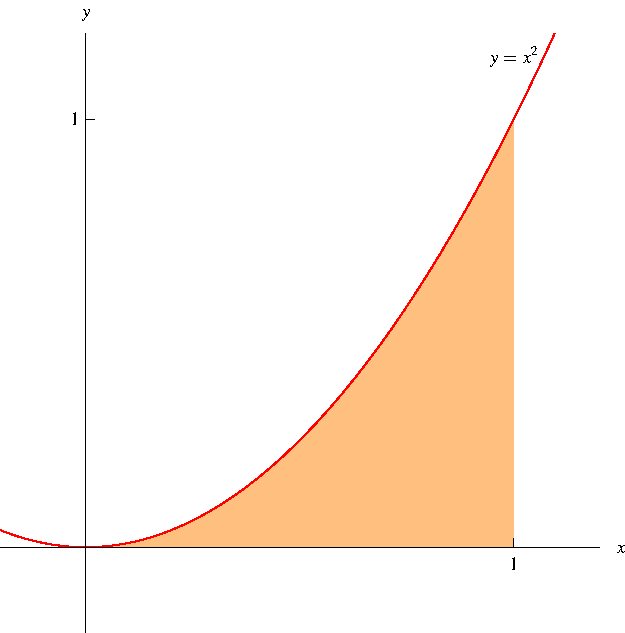
\includegraphics[height=4cm]{integration/pictures/05-01-xsquaredarea.pdf}%
}}%
\only<handout:6| 13>{%
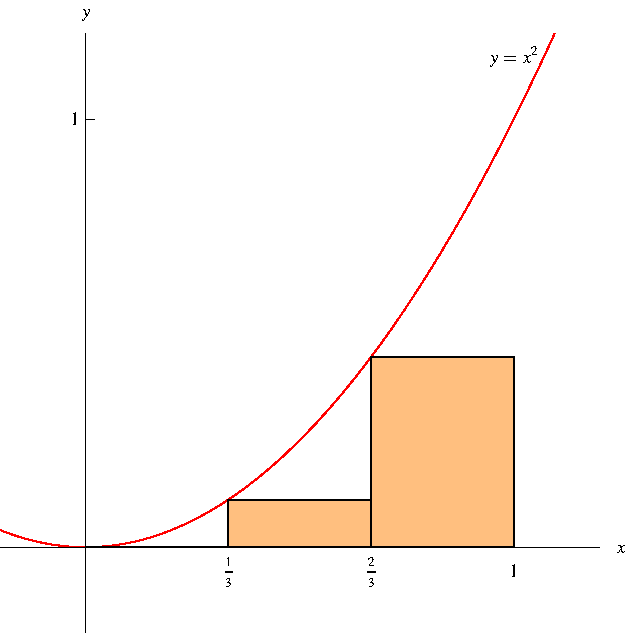
\includegraphics[height=4cm]{integration/pictures/05-01-lefta.pdf}%
}%
\only<handout:0| 14>{%
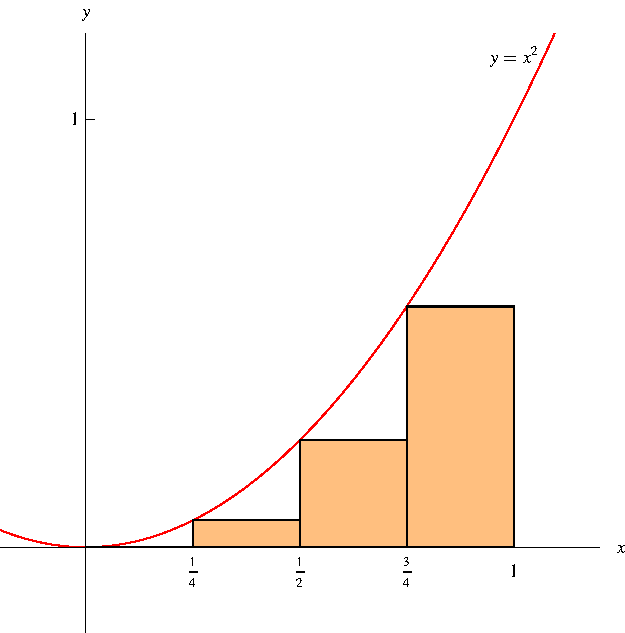
\includegraphics[height=4cm]{integration/pictures/05-01-leftb.pdf}%
}%
\only<handout:0| 15>{%
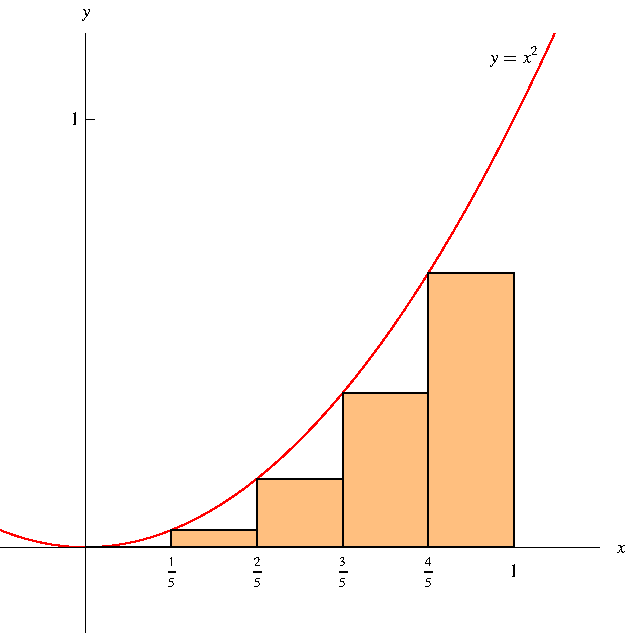
\includegraphics[height=4cm]{integration/pictures/05-01-leftc.pdf}%
}%
\only<handout:0| 16>{%
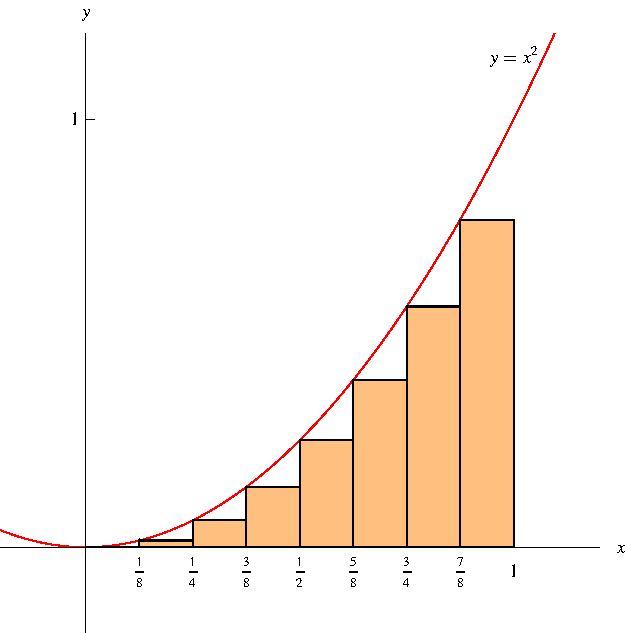
\includegraphics[height=4cm]{integration/pictures/05-01-leftd.pdf}%
}%
\only<handout:0| 17>{%
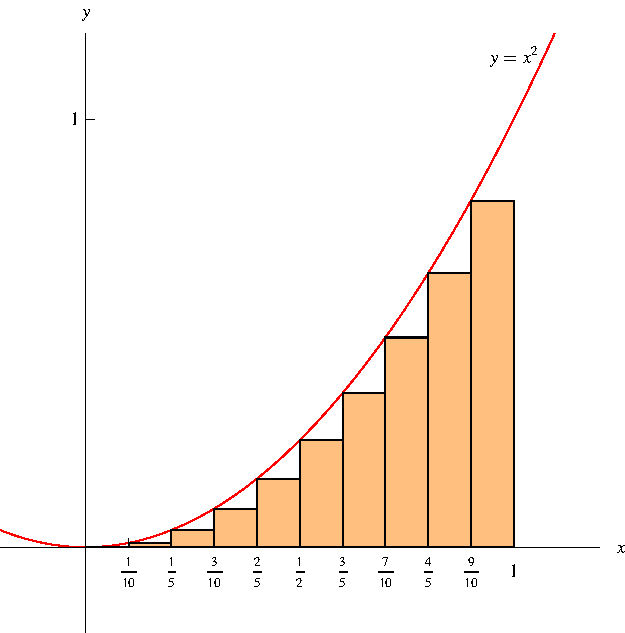
\includegraphics[height=4cm]{integration/pictures/05-01-lefte.pdf}%
}%
\only<handout:0| 18>{%
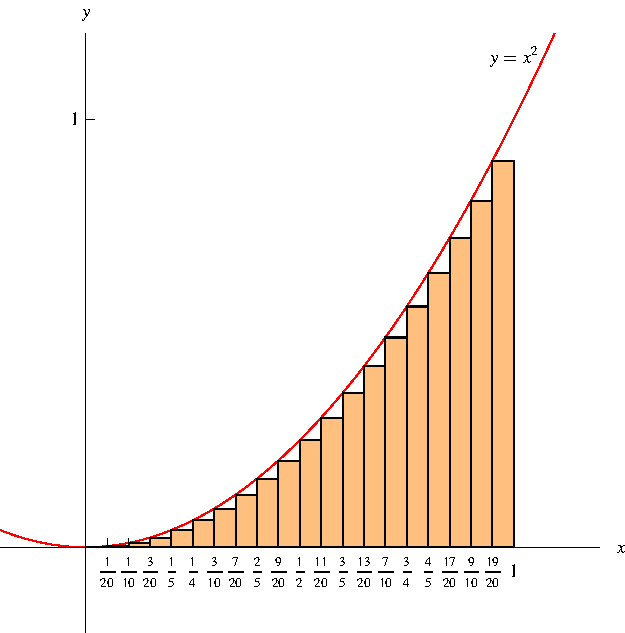
\includegraphics[height=4cm]{integration/pictures/05-01-leftf.pdf}%
}%
\only<handout:0| 19>{%
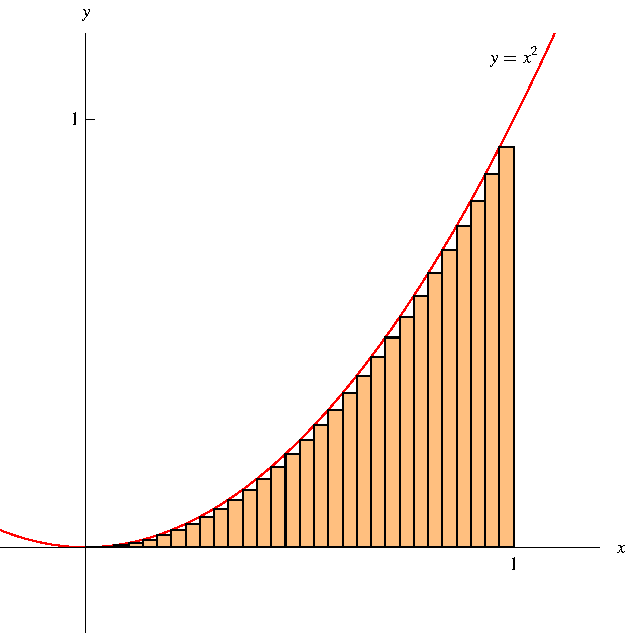
\includegraphics[height=4cm]{integration/pictures/05-01-leftg.pdf}%
}%
\only<handout:7| 20->{%
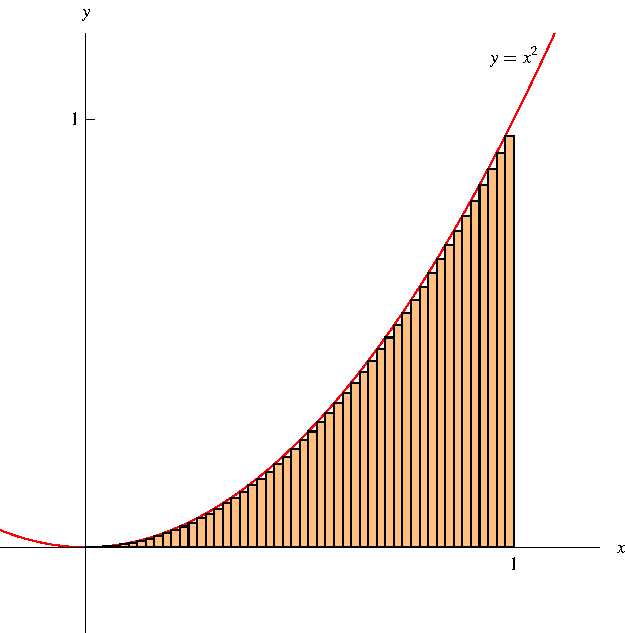
\includegraphics[height=4cm]{integration/pictures/05-01-lefth.pdf}%
}%
\ \only<handout:1| -2>{%
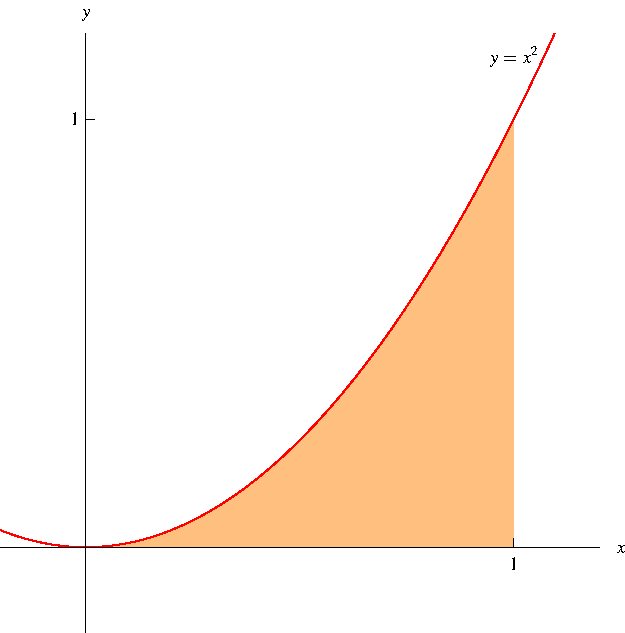
\includegraphics[height=4cm]{integration/pictures/05-01-xsquaredarea.pdf}%
}%
\only<handout:2| 3>{%
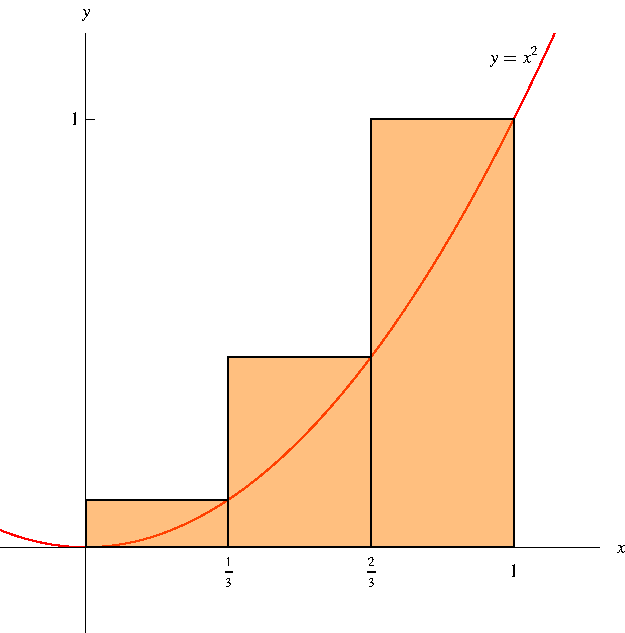
\includegraphics[height=4cm]{integration/pictures/05-01-righta.pdf}%
}%
\only<handout:3| 4>{%
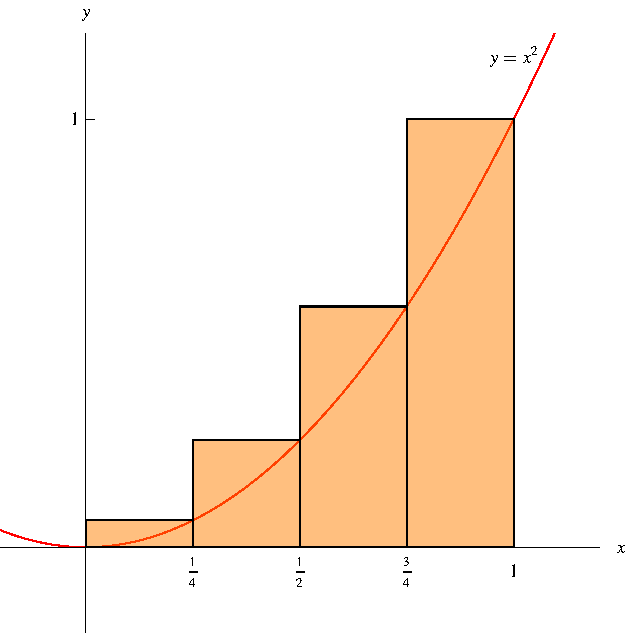
\includegraphics[height=4cm]{integration/pictures/05-01-rightb.pdf}%
}%
\only<handout:0| 5>{%
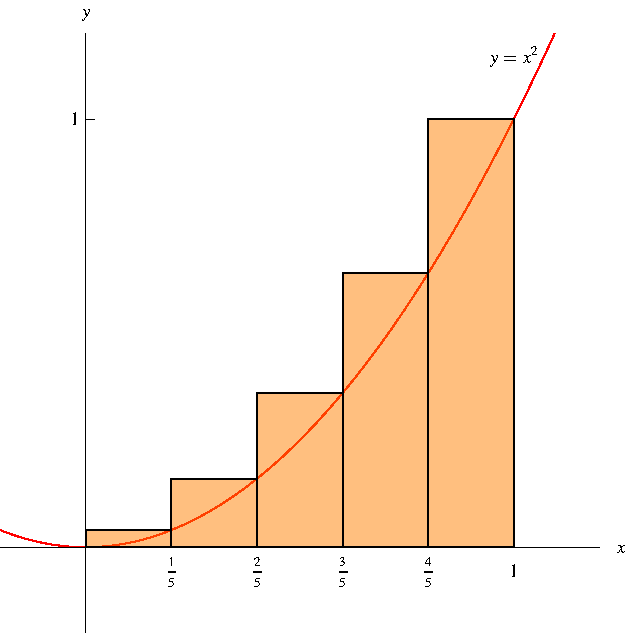
\includegraphics[height=4cm]{integration/pictures/05-01-rightc.pdf}%
}%
\only<handout:4| 6>{%
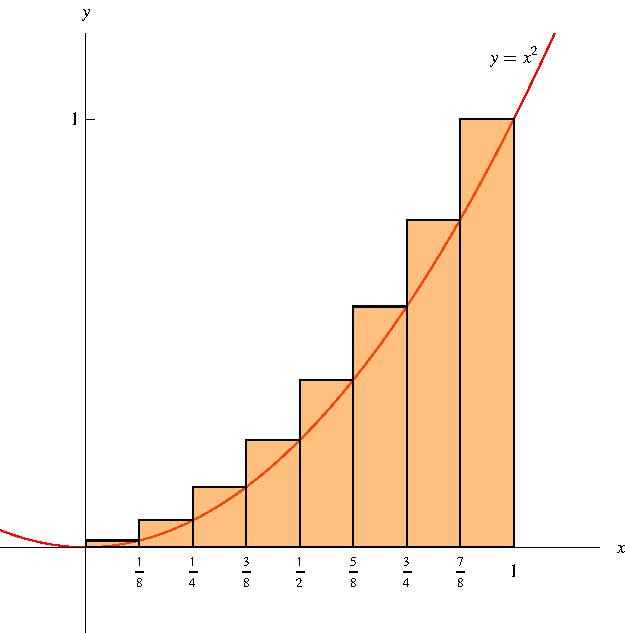
\includegraphics[height=4cm]{integration/pictures/05-01-rightd.pdf}%
}%
\only<handout:0| 7>{%
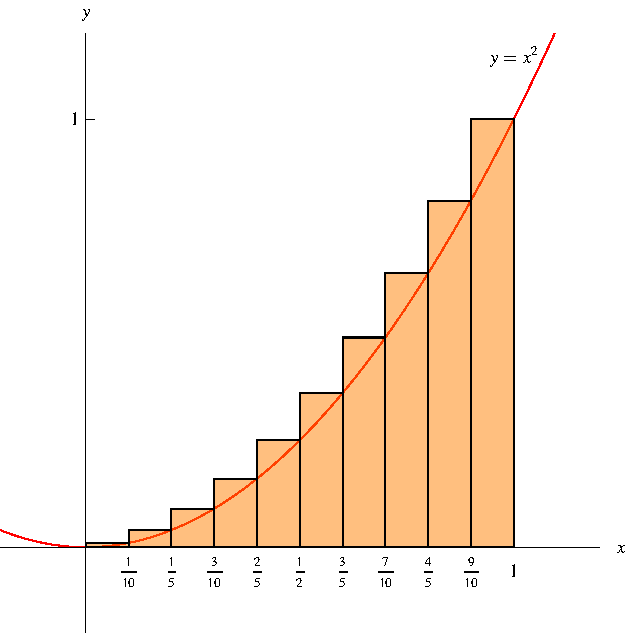
\includegraphics[height=4cm]{integration/pictures/05-01-righte.pdf}%
}%
\only<handout:0| 8>{%
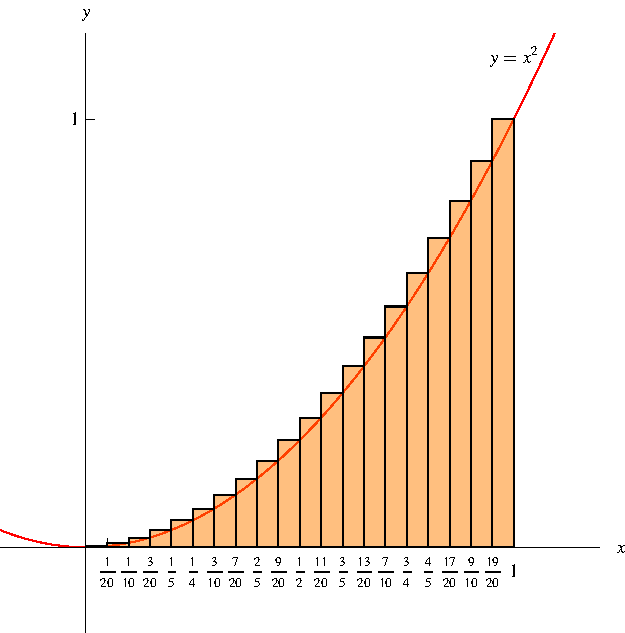
\includegraphics[height=4cm]{integration/pictures/05-01-rightf.pdf}%
}%
\only<handout:0| 9>{%
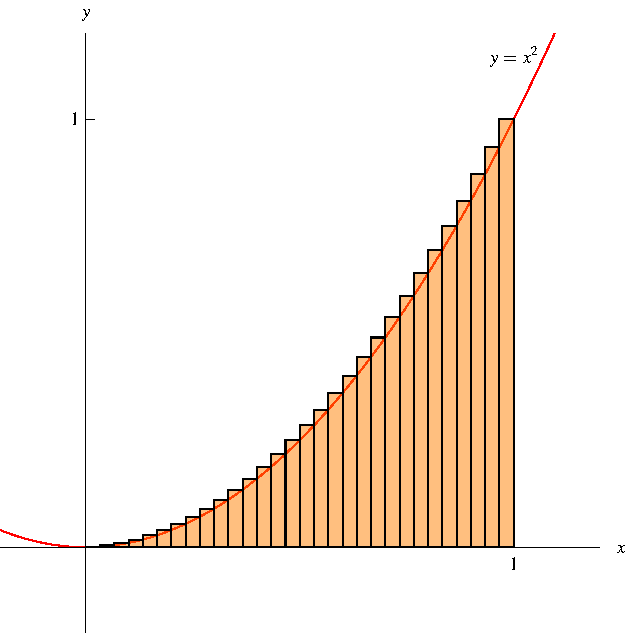
\includegraphics[height=4cm]{integration/pictures/05-01-rightg.pdf}%
}%
\only<handout:5-| 10->{%
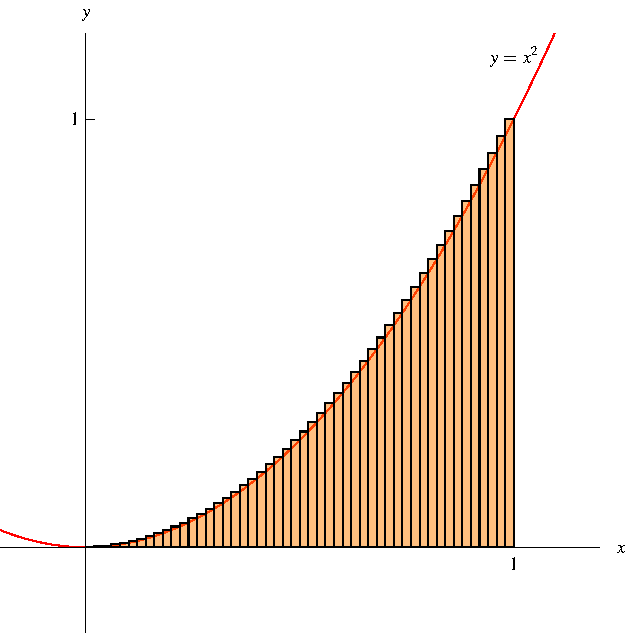
\includegraphics[height=4cm]{integration/pictures/05-01-righth.pdf}%
}%
\end{frame}
% end module areas-intro

%begin module area-under-hyperbola-ex1

\begin{frame}
Recall Euler substitution: $x=\frac12\left(\frac{1}{t}- t \right)$, $\alert<2>{\sqrt{x^2+1}=\frac{1}2\left(\frac 1 t +t\right)}$, $\alert<12,13,14>{ t=\sqrt{x^2+1}-x} $, $\alert<3>{ \diff x=-\frac12 \left(\frac1{t^2} +1\right)\diff t}$.
\begin{example}
$
\begin{array}{rcl}
\displaystyle \int \alert<2>{ \sqrt{x^2+1}} \alert<3>{\diff x} \vphantom{ \frac{1}{8}\left(\frac{1}{ (\sqrt{ x^2 +1} -x)^2} - (\sqrt{x^2+1}- x)^2 \right) } &=&
\displaystyle
\only<1-16>{
\uncover<2->{ \alert<3>{-} \int  \alert<2>{\alert<4>{\frac12} \left(\alert<5,6>{\frac1t} +\alert<7,8>{t}\right)} \alert<3>{\alert<4>{ \frac{1}{2}} \left(\alert<5,7>{ \frac 1 {t^2}} +\alert<6,8>{1} \right)\diff t}} \\
\uncover<4->{ &=&\displaystyle -\alert<4>{ \frac 1 4} \alert<9,10,11>{ \int} \left(\alert<5>{ \alert<9>{ \frac{ 1 }{ t^3}}} + \alert<6,7,10>{2\frac{1}t} + \alert<8,11>{t} \right) \alert<9,10,11>{ \diff t} } \\
\uncover<9->{&=&\displaystyle \alert<15>{-\frac{1}4} \left( \alert<9>{ \alert<15>{ -}\frac{ \alert<12>{ t^{-2}}}{\alert<15>{2}}} +\alert<10>{ \alert<15>{2} \ln\alert<14>{ |t|} }+ \alert<11>{\frac{\alert<13>{ t^2}}{\alert<15>{2}}} \right)+C}\\
\uncover<12->{&=&}
}
\uncover<12->{\displaystyle \only<1-24>{  \alert<16,17,18,24>{ \alert<15>{\frac{1}{8}} \left(\frac{1}{\alert<12>{ (\sqrt{ x^2 +1} -x)^2}} - \alert<13>{\left(\sqrt{x^2+1}- x\right)^2} \right) } }}\only<25->{
\alert<25>{ \frac{1}{2}x\sqrt{x^2+1}}
} {~~~~~~~~~~~~~~~~~~~~~~~~~~~~~~~~~~~~~~~~~~~~~~~~~~~~~~}  \\
\uncover<12->{ && \displaystyle \alert<16,17>{ \only<1-30>{\alert<15>{ -}} \only<31->{\alert<31>{+} } \alert<15>{ \frac12}  \alert<26,30>{\ln \left( \alert<14>{ \sqrt{x^2+1} \only<1-30>{-}\only<31->{\alert<31>{+} } x} \right)} +C}}
\end{array}
$

\noindent \only<17-25>{The answer is good. However, let's simplify.

\noindent
\uncover<18->{
$
\begin{array}{l}
\phantom{=}
\displaystyle \alert<18>{ \frac{1}{(\sqrt{x^2+1}-x)^2}- \left( \sqrt{ x^2+1 }-x\right)^2} \\
\uncover<19->{= \displaystyle \frac{ \alert<19>{(\sqrt{x^2+1} +x )^2} }{ ( \sqrt{x^2 +1} -x )^2  	\alert<19>{(\sqrt{x^2+1}+x)^2} } - \left(\sqrt{x^2+1}-x\right)^2} \\
\uncover<20->{ =\displaystyle \frac{(\sqrt{x^2+1}+x)^2}{ \alert<20>{ \alert<21,22>{((\sqrt{x^2 +1 } )^2 -x^2 )^2 } \uncover<21,22>{\alert<21,22>{=1}} } } - \left( \sqrt{x^2 +1 } -x \right)^2} \\
\displaystyle \uncover<22->{=\left(\sqrt{x^2+1}+x\right)^2-\left( \sqrt{ x^2 + 1 } -x\right)^2} \uncover<23->{ = \alert<24,25>{ 4x\sqrt{x^2+1}}}
\end{array}
$
} %uncover<18->
} %only<17-25>

\only<26->{
The last expression can be transformed to:
\[
\begin{array}{rcl}
\displaystyle
\alert<26>{\ln} \left(\frac{\alert<26,28>{\left(\sqrt{x^2+1}-x\right)} \uncover<27->{ \alert<27,28>{\left( \sqrt{x^2+1}+ x \right)} }}{ \uncover<27->{ \alert<27>{ \sqrt{x^2 +1} +x}}} \right)
&=& \displaystyle \uncover<28->{\alert<29>{ \ln \left( \frac{\alert<28>{ 1} }{ \sqrt{x^2+1}+x}\right)} }\\ \uncover<29->{&=&\alert<29,30,31>{ -\ln \left(\sqrt{x^2+1}+x\right)}}
\end{array}
\]
}
\end{example}

\vspace{8cm}
\end{frame}

\begin{frame}
\begin{example}
Find the area locked b-n the hyperbolas $\alert<2,3>{ y=\pm \sqrt{ x^2+1}}$ and $x=\pm 2\sqrt{ 2}$.
\begin{columns}
\column{.5\textwidth}
\psset{xunit=0.7cm, yunit=0.7cm}
\begin{pspicture}(-3.328427, -3)(3.328427,3)
\psframe*[linecolor=white](-3.328427,-3)(3.328427,3)
\tiny
\uncover<31->{
\pscustom*[linecolor=\fcColorAreaUnderGraph]{
\psplot[linecolor=\fcColorGraph, plotpoints = 1000 ] {-2.828427} {2.828427}{1 x 2 exp add 0.5 exp }
\psline[linecolor=\fcColorGraph](2.828427,-3)(2.828427,3)
\psplot[linecolor=\fcColorGraph, plotpoints=1000] { 2.828427 } {-2.828427}{1 x 2 exp add 0.5 exp -1 mul }
\psline[linecolor=\fcColorGraph](-2.828427,-3)(-2.828427,3)
}
}
\uncover<1-26,28->{
\psaxes[arrows=<->,ticks=none, labels=none](0,0)(-3,-3)(3,3)
}
\psline[linecolor=red!1](3.301,2)(3.302,2)
\psline[linecolor=red!1](-3.301,2)(-3.302,2)

%Function formula: - (x^{2}+1)^{1/2}
\psplot[linecolor=\fcColorGraph, plotpoints=1000]{-2.828427}{2.828427}{1 x 2 exp add 0.5 exp -1 mul }
\uncover<3-4>{\rput[tl](-2.2, -2.4){ \alert<3>{ $y= - \sqrt{ x^2 +1 }$}}}

%Function formula: (x^{2}+1)^{1/2}
\psplot[linecolor=\fcColorGraph, plotpoints=1000]{-2.828427}{ 2.828427 }{1 x 2 exp add 0.5 exp }
\uncover<2-4>{\rput[bl](-2.1, 2.4){\alert<2>{ $y=\sqrt{ x^2 +1} $}}}

\uncover<29->{
\psline[linecolor=\fcColorGraph](-2.828427,3)(-2.828427,-3)
}
\uncover<30->{
\psline[linecolor=\fcColorGraph](2.828427,3)(2.828427,-3)
}
\uncover<25-27>{
\psline{<->}(-2.9,2.9)(2.9,-2.9)
\rput[t](-2.1, 1.7){$\begin{array}{l} \alert<25>{v=0} \\\uncover<1-26>{\alert<25>{y+x=0}} \end{array}$}
}
\uncover<15-27>{
\psline{<->}(-2.9,-2.9)(2.9,2.9)
\rput[b](-2.1, -1.9){$\begin{array}{l} \uncover<1-26>{ \alert<15>{ y-x=0 }}\\\uncover<16->{\alert<16>{u=0}} \end{array}$}
}
\uncover<17-26>{
\fcFullDot{1.4}{1.4}
\rput[l]( 1.6, 1.4){$(\frac{y+x}{2},\frac{y+x}{2})$}
}
\uncover<14-26>{
\fcFullDot{0.6}{2.2}
\rput[lb](0.65, 2.2){$(x,y)$}
}
\uncover<26>{
\psline(0.6,2.2)(-0.8,0.8)
\psline(-0.7, 0.9)(-0.6, 0.8)(-0.7, 0.7)
\rput[rb](-0.3, 1.3){\alert<26>{$v$}}
}
\uncover<18-26>{
\psline(0.6,2.2)(1.4, 1.4)
\psline(1.3, 1.5)(1.2,1.4)(1.3, 1.3)
}
\uncover<23-26>{
\rput[tr](0.95, 1.8){\alert<23>{$u$}}
}
\uncover<14-26>{
\fcFullDot{2.2}{0.6}
\rput[lt]( 2.2, 0.65){$(y,x)$}
}
\end{pspicture}

\vbox to 3.0cm {
\uncover<18->{\alert<18>{
\uncover<22->{\alert<22>{Signed}} distance b-n $(x,y)$ and line $u=0$ equals}}
\only<1-23>{
$\uncover<19->{\uncover<22->{\alert<22>{\pm}} \alert<19>{ \sqrt{ \alert<20>{ \left(x-\frac{(x+y)}{2} \right)^2+ \left( y- \frac{(x+y )}{2} \right)^2}}}}
$
$\uncover<20->{=\uncover<22->{\alert<22>{\pm}} \sqrt{ \alert<20>{ \frac{1}{2}(y-x)^2 }}} \uncover<21->{= \alert<21>{ \uncover<1-21>{\pm} \alert<23>{ \frac{\sqrt{2 }}{ 2 } ( y-x)}}} \uncover<23>{ \alert<23>{=}}$
} %only<1-23>
\uncover<23->{ \alert<23,24>{$u $}.}
\only<24->{\uncover<25->{
Similarly compute that \alert<26>{signed distance b-n $(x,y)$ and the \alert<25>{line $v=0$} equals $v$}.
\uncover<27->{$\Rightarrow$ $y^2-x^2=1$ is the \alert<27>{ hyperbola $v=\frac{1/2}{v}$} in the $(u,v)$-plane.}
}}

\vfil
} %vbox

\column {.5\textwidth}
\only<1-27>{
\uncover<4->{We studied $\alert<27>{v=\frac{1/2}{u}}$ is called a hyperbola:}\uncover<3->{ why do we call $y= \sqrt{ x^2 +1}$ hyperbola?} \uncover<5->{Compute:}
\[
\begin{array}{rcl}
\uncover<5->{\sqrt{x^2+1} &=& y}\\
\uncover<6->{ x^2+1 &=& y^2}\\
\uncover<7->{y^2-x^2&=&1}\\
\uncover<8->{\uncover<9>{\alert<9>{\frac{1}{2}}} \uncover<10->{\alert<10,11>{\frac{\sqrt{2}}{2}}} \alert<11>{(y-x)} \uncover<10->{\alert<10,12>{\frac{\sqrt{2}}{2}}} \alert<12>{(y+x)}&=&\uncover<9->{\alert<9>{\frac{1}{2}}} \uncover<8>{1}}\\
\uncover<11->{\alert<11>{u}\alert<12>{v}&=& \frac{1}{2}}\\
\uncover<13->{\alert<27>{v}&\alert<27>{=}& \alert<27>{\frac{1/2}{u}},}
\end{array}
\]
\uncover<11->{where $\begin{array}{|l}
\alert<11,16,23>{u=\frac{\sqrt{2}}{2} \left(y-x\right)}\\
\alert<12,25>{v=\frac{\sqrt{2}}{2}\left(y+x\right)}
\end{array}$. } \uncover<14->{Consider an arbitrary point $(x,y)$.}
} %only<1-27>
\only<28->{
The area in question is:
$
\begin{array}{l}
\displaystyle\phantom{=} \int \limits^{{{\uncover<28,29>{\alert<29>{ \textbf{?}}}\uncover<30->{\alert<30>{ 2\sqrt{2}}}}}}_{\uncover<28>{\alert<28>{\textbf{?}}}\uncover<29->{ -2\sqrt{2}}} 2\sqrt{x^2+1}\diff x \\
\displaystyle \uncover<32->{= \uncover<33->{\alert<33>{2}} \left[x\sqrt{x^2+1} \vphantom{\ln \left(\sqrt{x^2+1}+x\right) }\right.}\\
\displaystyle \uncover<32->{\left. \ln \left(\sqrt{x^2+1}+x\right)\right]^{2\sqrt{2}}_{\only<33->{\alert<33>{0}} \uncover<1-32>{-2\sqrt{2}}}}\\
\uncover<34->{=2\left(2\sqrt{2} \sqrt{(2\sqrt{2})^2+1}\right.} \\
\uncover<34->{\left.+ \ln \left(\sqrt{(2\sqrt{2})^2+1}+2\sqrt{2} \right) \right)}\\
\uncover<35->{=12\sqrt{2} +2\ln \left(3+2\sqrt{2}\right )}\\
\uncover<36->{\approx 20.496}
\end{array}
$
}
\end{columns}

\end{example}

\end{frame}

%end module area-under-hyperbola-ex1

%begin module improper-integral-type1-arctan-geometric-interpretation
%\begin{comment}
\begin{frame}[t]

\psset{xunit=2cm, yunit=2cm}
\begin{pspicture}(-3.1, -0.1)(3.1,1.2)
\psframe*[linecolor=white](-3.1,-0.1)(3.1,1.2)
\tiny
\psline[linecolor=red!1](0,1.2)(0.001,1.2) %bounding boxes don't always work right
\psaxes[arrows=<->, ticks=none, labels=none] (0,0) (-3.05,-0.1) (3.05,1.1)
\rput[t](3, -0.1){$x$}

%Function formula: - (- x^{2}+1)^{1/2}
%\psplot[linecolor=\fcColorGraph, plotpoints=1000]{-1}{1}{1 x 2 exp -1 mul add 0.5 exp -1 mul }
%Function formula: (- x^{2}+1)^{1/2}
\psplot[linecolor=blue, plotpoints=1000] {-1} {1} {1 x 2 exp -1 mul add 0.5 exp }
\psline(-3,1)(3,1)

\uncover<3->{
\psline{<-}(-0.05, 0)(-0.05,0.4)
\psline{->}(-0.05, 0.6)(-0.05,1)
\rput(-0.05, 0.5){\alertNoH{3}{$1$}}
}
\uncover<2>{
\psline[linecolor=red](0.5,1)(1,1)
\fcFullDot{1}{1}
}
\uncover<2>{
\fcFullDot{0.5}{1}
}

\rput[br](-0.05, 1.05){ $\phantom{Q_0=P_0}A$}
\uncover<2->{
\rput[lb](0.5, 1.05){$P_1\phantom{(x_1 ,1)}$}
\rput[lb](1, 1.05){$P_2(\alertNoH{2}{x_2}, 1)$}
}
\uncover<2->{
\rput[t](0.75,0.95){\alertNoH{2}{$\Delta$}}
}
\uncover<5->{
\rput[lt](0.520000, 0.4500000){$\alertNoH{5}{Q_2}$}
\rput[l](0.42000, 0.8){$\alertNoH{5}{Q_1}$}
}
\rput[tl](0.05, -0.05){$O$}
%calculator commands:
%\Delta:=0.5;
%xInv{}{{x}}:=DoubleValue{}x/(1+x^2);
%yInv{}{{x}}:=DoubleValue{} 1/(1+x^2);
%xDir{}{{x}}:=-xInv{}x;
%yDir{}{{x}}:=1-yInv{}x;
%lengthN{}{{x}}:=((xDir{}x)^2+(yDir{}x)^2)^{1/2};
%xDirN{}{{x}}:=0.05 xDir{}x /lengthN{}x ;
%yDirN{}{{x}}:=0.05 yDir{}x/lengthN{}x;
%xT{}{{x}}:=-yDirN{}x;
%yT{}{{x}}:=xDirN{}x;

%inversePoint{}{{x}}:=(xInv{}x,yInv{}x );
%f{}{{x}}:= \psline(DoubleValue{}x,1 )(0,0) \psline inversePoint{}x (0,1)  \psline inversePoint{}x inversePoint{}(x+\Delta) \psline (xInv{}x +xDirN{}x, yInv{}x+yDirN{}x ) (xInv{}x +xDirN{}x+xT{}x, yInv{}x+yDirN{}x +yT{}x)(xInv{}x +xT{}x, yInv{}x +yT{}x);
%f{}(\Delta) f{}(2\Delta)f{}(3\Delta)f{}(4\Delta)f{}(5\Delta)f{}(6\Delta)

\uncover<5->{
\psline (0.5, 1) (0, 0)
}
\uncover<5->{
\psline (0.4, 0.8) (0, 1)
}
\uncover<15->{
\psline (0.4, 0.8) (0.5, 0.5)
}
\uncover<5->{\psline (0.355279, 0.822361) (0.332918, 0.777639) (0.377639, 0.755279) }

\uncover<4->{\psline (1, 1) (0, 0) }
\uncover<5->{\psline (0.5, 0.5) (0, 1)}
%\psline (0.5, 0.5) (0.461538, 0.307692)
\uncover<5->{\psline (0.464645, 0.535355) (0.429289, 0.5) (0.464645, 0.464645) }


%\psline (1.500000, 1) (0, 0)
%\psline (0.461538, 0.307692) (0, 1)
%\psline (0.461538, 0.307692) (0.4, 0.2)
%\psline (0.433803, 0.349295) (0.392201, 0.321560) (0.419936, 0.279957)

%\psline (2, 1) (0, 0)
%\psline (0.4, 0.2) (0, 1)
%\psline (0.4, 0.2) (0.344828, 0.137931)
%\psline (0.377639, 0.244721) (0.332918, 0.222361) (0.355279, 0.177639)

%\psline (2.5, 1) (0, 0)
%\psline (0.344828, 0.137931) (0, 1)
%\psline (0.344828, 0.137931) (0.300000, 0.100000)
%\psline (0.326258, 0.184355) (0.279834, 0.165785) (0.298404, 0.119362)

%\psline (3, 1) (0, 0)
%\psline (0.300000, 0.100000) (0, 1)
%\psline (0.300000, 0.100000) (0.264151, 0.075472)
%\psline (0.284189, 0.147434) (0.236754, 0.131623) (0.252566, 0.084189)

%\psline (-0.5, 1) (0, 0)
%\psline (-0.4, 0.8) (0, 1)
%\psline (-0.4, 0.8) (-0.5, 0.5) \psline (-0.355279, 0.822361) (-0.377639, 0.867082) (-0.422361, 0.844721)

%\psline (-1, 1) (0, 0)
%\psline (-0.5, 0.5) (0, 1)
%\psline (-0.5, 0.5) (-0.461538, 0.307692)
%\psline (-0.464645, 0.535355) (-0.5, 0.570711) (-0.535355, 0.535355)

%\psline (-1.500000, 1) (0, 0)
%\psline (-0.461538, 0.307692) (0, 1)
%\psline (-0.461538, 0.307692) (-0.4, 0.2)
%\psline (-0.433803, 0.349295) (-0.475406, 0.377030) (-0.503141, 0.335427)

%\psline (-2, 1) (0, 0)
%\psline (-0.4, 0.2) (0, 1)
%\psline (-0.4, 0.2) (-0.344828, 0.137931)
%\psline (-0.377639, 0.244721) (-0.422361, 0.267082) (-0.444721, 0.222361)

%\psline (-2.5, 1) (0, 0)
%\psline (-0.344828, 0.137931) (0, 1)
%\psline (-0.344828, 0.137931) (-0.300000, 0.100000)
%\psline (-0.326258, 0.184355) (-0.372682, 0.202924) (-0.391251, 0.156501)

%\psline (-3, 1) (0, 0)
%\psline (-0.300000, 0.100000) (0, 1)
%\psline (-0.300000, 0.100000) (-0.264151, 0.075472)
%\psline (-0.284189, 0.147434) (-0.331623, 0.163246) (-0.347434, 0.115811)


%Function formula: - (- x^{2}+1/4)^{1/2}+1/2
%\psplot[linecolor=blue, plotpoints=1000]{-0.5}{0.5}{0.5 0.2500000 x 2 exp -1 mul add 0.5 exp -1 mul add }

%Function formula: (- x^{2}+1/4)^{1/2}+1/2
%\psplot[linecolor=blue, plotpoints=1000]{-0.5}{0.5}{0.5 0.2500000 x 2 exp -1 mul add 0.5 exp add }

\uncover<3,6>{
\psline[linecolor=red](1, 1) (0, 0)(0,1)(1,1)
}
\uncover<4>{
\psline[linecolor=red](0.5, 1) (0, 0)(0,1)(0.5,1)
}

\uncover<7>{
\psline[linecolor=red](0.5, 0.5) (0, 0)(0,1)(0.5,0.5)
}
\uncover<8>{
\psline[linecolor=green](0,0)(0,1)
\psline[linecolor=red](0,0)(1,1)
}
\uncover<9>{
\psline[linecolor=green](0,0)(0.5,0.5)
\psline[linecolor=red](0,0)(0,1)
}
\uncover<15>{
\psline[linecolor=red](0,0)(0.5, 0.5)(0.4,0.8)(0,0)
}
\uncover<16>{
\psline[linecolor=red](0,0)(1, 1)(0.5,1)(0,0)
}
\uncover<17,18>{
\psline[linecolor=green](0.5, 0.5)(0.4, 0.8)
\psline[linecolor=red](0.5, 1)(1, 1)
}
\uncover<18>{
\psline[linecolor=green](0.5, 0.5)(0.0, 0.0)
\psline[linecolor=red](0, 0)(0.5, 1)
}
\end{pspicture}
\only<handout:1|1-26>{
Draw a unit circle as above, let $O, A$ be as indicated. \uncover<2->{Let $P_2$ be the point $(\alertNoH{2}{x_2},1)$, $P_1$ be the point $(x_2-\alertNoH{2}{\Delta},1)$.} \uncover<3->{By the Pythagorean theorem, $\alertNoH{25}{|OP_2|^2= 1 + x_2^2}$} \uncover<4->{and similarly $ |OP_1 |^2=1+(x_2-\Delta )^2$.} \uncover<5->{Let \alertNoH{5}{$Q_1$}, \alertNoH{5}{$Q_2$} be as indicated.} \uncover<6->{Then $\alertNoH{6}{ \triangle OP_2A} $ is similar to $\alertNoH{7}{\triangle OAQ_2} $.} \uncover<8->{By Euclidean geometry, $\alertNoH{8}{ \frac{ \only<1-8>{{\color{green} |OA|}} \only<handout:0|9->{|OA|} }{ |OP_2| }} =\alertNoH{9}{ \frac{\only<9>{{\color{green}|OQ_2|}} \only<handout:0|8,10->{| OQ_2|} }{|OA|}}$} \uncover<10->{ and so $\alertNoH{12,24}{|OQ_2| |OP_2| }= |OA|^2 \alertNoH{12,24}{ =1}$ \uncover<23->{ and therefore $\alertNoH{23}{ \frac{|OQ_2|}{|OP_2|}} = \frac{ \alertNoH{24}{|OQ_2| \alertNoH{23}{| OP_2 |}} }{|OP_2|^{\alertNoH{23}{2} }} \uncover<24->{= \frac{ \alertNoH{24}{ 1} }{ \alertNoH{25}{|OP_2|^2}} } \uncover<25->{ = \frac{1}{\alertNoH{25}{ 1+x_2^2}}.}$}
}
%The points $Q_2$, $P_2$ are often called ``inverse points w.r.t. the unit circle''.
\uncover<11->{Similarly conclude $\alertNoH{13}{ |OQ_1|} \alertNoH{14}{|OP_1|} =|OA|^2= \alertNoH{12}{1} \uncover<12->{ \alertNoH{12}{\alertNoH{13,14}{=} \alertNoH{14}{ |OQ_2|}\alertNoH{13}{ |OP_2| }}.}$}
\uncover<13->{Therefore $\alertNoH{13}{ \frac{|OQ_1|}{  |OP_2|} } \alertNoH{13,14}{=} \alertNoH{14}{\frac{|OQ_2| }{ |OP_1|}} $} \uncover<15->{and so $ \alertNoH{15}{\triangle OQ_2Q_1} $ is similar to $\alertNoH{16}{\triangle OP_1P_2} $.} \uncover<17->{Therefore $\frac{ \only<17>{{ \color{green}|Q_1Q_2|}} \only<handout:0|18->{\alertNoH{19}{ |Q_1Q_2|}} } { \alertNoH{17,20}{|P_1P_2|} }= \alertNoH{20}{ \frac{ \only<18>{\color{green}|OQ_2|} \only<handout:0| 1-17,19->{ |OQ_2|} }{ \alertNoH{18}{|OP_1|} }}$} \uncover<19->{and so }
}
\uncover<19->{\alertNoH{26,27}{\noindent $\alertNoH{19}{|Q_1Q_2|} =\alertNoH{20}{\frac{|P_1P_2| |OQ_2|} {|OP_1|}} \uncover<21->{=\left(\frac{\alertNoH{21}{|OP_2|} }{|OP_1|}\right) \alertNoH{23,24,25}{\frac{|OQ_2|} {\alertNoH{21}{ |OP_2|}}} \alertNoH{22}{ |P_1P_2|} } \uncover<22->{= \frac{|OP_2| } {|OP_1|} \frac{\alertNoH{22}{ \Delta} }{\alertNoH{23,24,25}{ 1+x_2^2}}.}$}}
\end{frame}
%\end{comment}
%\begin{comment}
\begin{frame}[t]
\psset{xunit=2cm, yunit=2cm}
\begin{pspicture}(-3.1, -0.1)(3.1,1.2)
\psframe*[linecolor=white](-3.1,-0.1)(3.1,1.2)
\tiny
\psline[linecolor=red!1](0,1.2)(0.001,1.2) %bounding boxes don't always work right
%\uncover<48->{
%\pscustom*[linecolor=\fcColorAreaUnderGraph]{
%Function formula: \frac{1}{x^{2}+1}
%\psplot[linecolor=\fcColorGraph, plotpoints=1000]{-3.000000}{3.000000}{1.0000000 1.0000000 x 2.0000000 exp add div }
%\psline(3.000000, 0)(-3.000000, 0)
%}

%Function formula: \frac{1}{x^{2}+1}
%\psplot[linecolor=\fcColorGraph, plotpoints=1000]{-3.000000} {3.000000} {1.0000000 1.0000000 x 2.0000000 exp add div }
%}

\psaxes[arrows=<->, ticks=none, labels=none](0,0)(-3.05,-0.1)(3.05,1.1)
%Function formula: - (- x^{2}+1)^{1/2}
%\psplot[linecolor=\fcColorGraph, plotpoints=1000]{-1}{1}{1 x 2 exp -1 mul add 0.5 exp -1 mul }
%Function formula: (- x^{2}+1)^{1/2}
\psplot[linecolor=blue, plotpoints=1000]{-1}{1}{1 x 2 exp -1 mul add 0.5 exp }
\psline(-3,1)(3,1)
%calculator commands:
%\Delta:=0.5;
%xInv{}{{x}}:=DoubleValue{}x/(1+x^2);
%yInv{}{{x}}:=DoubleValue{} 1/(1+x^2);
%xDir{}{{x}}:=-xInv{}x;
%yDir{}{{x}}:=1-yInv{}x;
%lengthN{}{{x}}:=((xDir{}x)^2+(yDir{}x)^2)^{1/2};
%xDirN{}{{x}}:=0.05 xDir{}x /lengthN{}x ;
%yDirN{}{{x}}:=0.05 yDir{}x/lengthN{}x;
%xT{}{{x}}:=-yDirN{}x;
%yT{}{{x}}:=xDirN{}x;

%inversePoint{}{{x}}:=(xInv{}x,yInv{}x );
%f{}{{x}}:= \psline(DoubleValue{}x,1 )(0,0) \psline inversePoint{}x (0,1)  \psline inversePoint{}x inversePoint{}(x+\Delta) \psline (xInv{}x +xDirN{}x, yInv{}x+yDirN{}x ) (xInv{}x +xDirN{}x+xT{}x, yInv{}x+yDirN{}x +yT{}x)(xInv{}x +xT{}x, yInv{}x +yT{}x);
%f{}(\Delta) f{}(2\Delta)f{}(3\Delta)f{}(4\Delta)f{}(5\Delta)f{}(6\Delta)

\uncover<1-33>{
\psline(0.5, 1)(0, 0)
}
\uncover<34-41>{
\psline(0.4, 0.8)(0, 0)
}
\psline(0.4, 0.8)(0, 1)
\uncover<28,34>{
\psline[linecolor=red](0.4, 0.8)(0, 1)
}
\uncover<1-41>{
\psline(0.355279, 0.822361)(0.332918, 0.777639)(0.377639, 0.755279)
}
\uncover<22>{
\psline[linecolor=red](0.4, 0.8)(0, 1)
\psline[linecolor=red](0.355279, 0.822361)(0.332918, 0.777639)(0.377639, 0.755279)
}
\uncover<7-12>{
\psline(0.600000, 1)(0, 0)
\psline(0.441176, 0.735294)(0, 1)
\psline(0.441176, 0.735294)(0.4, 0.8)
\psline(0.398302, 0.761019)(0.372577, 0.718144)(0.415452, 0.692419)
}
\rput[lt](0.46, 0.71){\uncover<handout:0|7-12>{$Q_2$}}
\uncover<6>{
\psline(0.700000, 1)(0, 0)
\psline(0.469799, 0.671141)(0, 1)
\psline(0.469799, 0.671141)(0.4, 0.8)
\psline(0.428837, 0.699814)(0.400164, 0.658852)(0.441126, 0.630179)
}
\rput[lt](0.48, 0.65){\uncover<handout:0|6>{$Q_2$}}
\uncover<5>{
\psline(0.8, 1)(0, 0)
\psline(0.487805, 0.609756)(0, 1)
\psline(0.487805, 0.609756)(0.4, 0.8)
\psline(0.448761, 0.640991)(0.417527, 0.601947)(0.456570, 0.570713)
}
\rput[lt](0.5, 0.58){\uncover<handout:0|5>{$Q_2$}}
\uncover<4>{
\psline(0.900000, 1) (0, 0)
\psline(0.497238, 0.552486)(0, 1)
\psline(0.497238, 0.552486)(0.4, 0.8)
\psline(0.460073, 0.585934)(0.426625, 0.548770)(0.463789, 0.515321)
}
\rput[lt](0.5, 0.54){\uncover<handout:0|4>{$Q_2$}}

\uncover<1-3>{ %
\psline(1, 1)(0, 0)
\psline(0.4, 0.8)(0.5, 0.5)
} %
\rput[lt](0.520000, 0.4500000){\uncover<1-3>{$Q_2$}}
\uncover<13->{ %
\psline(0.4, 0.8)(0.5, 0.5)
} %
\rput[lt](0.520000, 0.4500000){\uncover<handout:0|13->{$Q_2$}}
\uncover<13-33>{ %
\psline(1, 1)(0, 0)
}
\uncover<34-41>{
\psline(0.5, 0.5)(0, 0)
}
\uncover<30,34>{
\psline[linecolor=red](0.4, 0.8)(0.5, 0.5)
}
\uncover<32->{
\psline(0.5, 0.5)(0.461538, 0.307692)
}
\uncover<32,34>{
\psline[linecolor=red](0.5, 0.5)(0.461538, 0.307692)
}
\uncover<1-3, 13-41>{
\psline(0.5, 0.5)(0, 1)
\psline(0.464645, 0.535355)(0.429289, 0.5)(0.464645, 0.464645)
}
\uncover<23>{
\psline[linecolor=red](0.5, 0.5)(0, 1)
\psline[linecolor=red](0.464645, 0.535355)(0.429289, 0.5)(0.464645, 0.464645)
}
\uncover<14>{ %
\psline[linecolor=red](0,0)(0,1)
} %
\uncover<15>{
\psline[linecolor=red](0,0)(0.5,1)
}
\uncover<16>{
\psline[linecolor=red](0,0)(1,1)
}
\uncover<17-33>{
\psline(1.5, 1)(0, 0)
}
\uncover<34-41>{
\psline(0.461538, 0.307692)(0, 0)
}
\uncover<17>{
\psline[linecolor=red](1.500000, 1)(0, 0)
}
\uncover<32->{
\psline(0.461538, 0.307692)(0.4, 0.2)
}
\uncover<32,34>{
\psline[linecolor=red](0.461538, 0.307692)(0.4, 0.2)
}
\uncover<24-41>{
\psline(0.461538, 0.307692)(0, 1)
\psline(0.433803, 0.349295)(0.392201, 0.321560)(0.419936, 0.279957)
}
\uncover<24>{
\psline[linecolor=red](0.461538, 0.307692)(0, 1)
\psline[linecolor=red](0.433803, 0.349295)(0.392201, 0.321560)(0.419936, 0.279957)
}
\uncover<18-33>{
\psline(2, 1)(0, 0)
}
\uncover<34-41>{
\psline(0.4, 0.2)(0, 0)
}
\uncover<18>{
\psline[linecolor=red](2, 1)(0, 0)
}
\uncover<32->{
\psline(0.4, 0.2)(0.344828, 0.137931)
}
\uncover<32,34>{
\psline[linecolor=red](0.4, 0.2)(0.344828, 0.137931)
}
\uncover<25-41>{
\psline(0.4, 0.2)(0, 1)
\psline(0.377639, 0.244721)(0.332918, 0.222361)(0.355279, 0.177639)
}
\uncover<25>{
\psline[linecolor=red](0.4, 0.2)(0, 1)
\psline[linecolor=red](0.377639, 0.244721)(0.332918, 0.222361)(0.355279, 0.177639)
}
\uncover<19-33>{
\psline(2.5, 1)(0, 0)
}
\uncover<34-41>{
\psline(0.344828, 0.137931)(0, 0)
}
\uncover<19>{
\psline[linecolor=red](2.5, 1)(0, 0)
}
\uncover<32->{
\psline(0.344828, 0.137931)(0.300000, 0.100000)
}
\uncover<32,33,34>{
\psline[linecolor=red](0.344828, 0.137931)(0.300000, 0.100000)
}
\uncover<26-41>{
\psline(0.344828, 0.137931)(0, 1)
\psline(0.326258, 0.184355)(0.279834, 0.165785)(0.298404, 0.119362)
}
\uncover<26>{
\psline[linecolor=red](0.344828, 0.137931)(0, 1)
\psline[linecolor=red](0.326258, 0.184355)(0.279834, 0.165785)(0.298404, 0.119362)
}
\uncover<20-33>{
\psline(3, 1)(0, 0)
}
\uncover<34-41>{
\psline(0.300000, 0.100000)(0, 0)
}
\uncover<20>{
\psline[linecolor=red](3, 1)(0, 0)
}
%\psline(0.300000, 0.100000)(0.264151, 0.075472)
\uncover<27-41>{
\psline(0.300000, 0.100000)(0, 1)
\psline(0.284189, 0.147434)(0.236754, 0.131623)(0.252566, 0.084189)
}
\uncover<27->{
\rput[lt](0.3,0.095){$Q_n$}
}
\uncover<27>{
\psline[linecolor=red](0.300000, 0.100000)(0, 1)
\psline[linecolor=red](0.284189, 0.147434)(0.236754, 0.131623)(0.252566, 0.084189)
}

\uncover<44>{
\psline(-0.5, 1)(0, 0)
\psline(-0.4, 0.8)(0, 1)
\psline(-0.355279, 0.822361)(-0.377639, 0.867082)(-0.422361, 0.844721)

\psline(-1, 1)(0, 0)
\psline(-0.5, 0.5)(0, 1)
\psline(-0.464645, 0.535355)(-0.5, 0.570711)(-0.535355, 0.535355)

\psline(-1.500000, 1) (0, 0)
\psline(-0.461538, 0.307692)(0, 1)
\psline(-0.433803, 0.349295)(-0.475406, 0.377030)(-0.503141, 0.335427)

\psline(-2, 1) (0, 0)
\psline(-0.4, 0.2)(0, 1)
\psline(-0.377639, 0.244721)(-0.422361, 0.267082)(-0.444721, 0.222361)

\psline(-2.5, 1) (0, 0)
\psline(-0.344828, 0.137931)(0, 1)
\psline(-0.326258, 0.184355)(-0.372682, 0.202924)(-0.391251, 0.156501)

\psline(-3, 1)(0, 0)
\psline(-0.300000, 0.100000)(0, 1)
%\psline (-0.300000, 0.100000) (-0.264151, 0.075472)
\psline(-0.284189, 0.147434)(-0.331623, 0.163246)(-0.347434, 0.115811)
}
\uncover<44->{
\psline(-0.4, 0.8)(-0.5, 0.5)
\psline(-0.5, 0.5)(-0.461538, 0.307692)
\psline(-0.461538, 0.307692)(-0.4, 0.2)
\psline(-0.4, 0.2)(-0.344828, 0.137931)
\psline(-0.344828, 0.137931)(-0.300000, 0.100000)
}

%Function formula: - (- x^{2}+1/4)^{1/2}+1/2
\uncover<42->{\psplot[linecolor=red, plotpoints=1000]{-0.5}{0.5}{0.5 0.2500000 x 2 exp -1 mul add 0.5 exp -1 mul add }

%Function formula: (- x^{2}+1/4)^{1/2}+1/2
\psplot[linecolor=red, plotpoints=1000]{-0.5}{0.5}{0.5 0.2500000 x 2 exp -1 mul add 0.5 exp add }
}
\uncover<8-12>{
\psline[linecolor=red](0,0)(0.6,1)
\psline[linecolor=green](0,0)(0.5,1)
}
\uncover<handout:0|4>{
\rput[lb](0.9, 1.05){$P_2$}
\rput[t](0.7,0.95){$\Delta$}
}
\uncover<handout:0|5>{
\rput[lb](0.8, 1.05){$P_2$}
\rput[t](0.65,0.95){$\Delta$}
}
\uncover<handout:0|6>{
\rput[lb](0.7, 1.05){$P_2$}
\rput[t](0.6,0.95){$\Delta$}
}
\uncover<handout:0|7-12>{
\rput[lb](0.6, 1.05){$P_2$}
\rput[t](0.55,0.95){$\Delta$}
}
\uncover<1-3,13->{
\rput[lb](1, 1.05){\uncover<1-33>{$P_2\alertNoH{16}{(x_2, 1)}$}}
\rput[t](0.75,0.95){$\Delta$}
}
\rput[rb](3, 1.05){$\uncover<20-33>{\alertNoH{20}{P_n}}$}
\rput[lb](2, 1.05){
$\uncover<17-33>{\alertNoH{17}{\dots}}$
}

\rput[lb](0.5, 1.05){\uncover<1-33>{$P_1\uncover<15->{\alertNoH{15}{(x_1 ,1)}}$}}
\rput[t](3, -0.1){$x$}
\rput[br](-0.05, 1.05){$\uncover<21->{\alertNoH{21}{Q_0= }}\uncover<14->{ \alertNoH{14}{ P_0=}}A$}
\rput[l](0.42000, 0.8){$Q_1$}
\rput[tl](0.05, -0.05){$O$}
\end{pspicture}
\alertNoH{1}{ \noindent $\alertNoH{28}{|Q_1Q_2| =} \alertNoH{29}{\frac{|OP_2| } {|OP_1|}} \alertNoH{28}{\frac{ \Delta} {1+x_2^2}}. \vphantom{={\frac{|P_1P_2| |OQ_2|} {|OP_1|}} {=\left(\frac{|OP_2|}{|OP_1|}\right) \frac{|OQ_2|} { |OP_2|} |P_1P_2| } }$} \uncover<13->{For any $\varepsilon >0$, can choose $\Delta$: $\alertNoH{29}{1< \frac{|OP_2| } {|OP_1|} < 1 + \varepsilon}$.}

\only<handout:1|1-12>{ \uncover<2->{If we let $P_2\to P_1$}\uncover<3->{, i.e., $\Delta \to 0$,} \uncover<8->{we get $\alertNoH{8}{ \frac{|OP_2| }{ |OP_1|}\to 1}$.} \uncover<9->{In strict mathematical language: for every $\varepsilon>0$ there exists $\delta >0$ such that when $\Delta  < \delta$ we have that $1>\frac{ |OP_2| }{|OP_1|}>1-\varepsilon $.} \uncover<10->{Furthermore, the choice of $\delta$ can be made independent of the value of $x_2$: } \uncover<11->{to prove that one analyzes the expression $\frac{|OP_2|}{|OP_1|} = \sqrt{ \frac{ 1+x_2^2} { 1 + (x_2-\Delta )^2}}$.} \uncover<12->{We leave the tedious but otherwise easy details to the interested student. }
}

\only<handout:2|13-27>{
\uncover<13->{Fix a large number $N$ and let $\Delta$ be such that $n= \frac{N}{\Delta} $ is integer.} \uncover<14->{ Let  $\alertNoH{14}{P_0=(0,1)} $, $\alertNoH{15}{P_1=(\Delta, 1 )}$, $\alertNoH{16}{P_2=(2\Delta,1)}, \dots, \alertNoH{20}{P_n= (n \Delta,1)}$}\uncover<21->{, and let $\alertNoH{21}{Q_0}, \alertNoH{22}{ Q_1},\alertNoH{23}{Q_2}, \dots, \alertNoH{27}{Q_n}$ be as indicated.}
}

\only<handout:3|28->{
$
\begin{array}{rcrcl}
\only<1-39>{
\alertNoH{28}{ \frac{\Delta}{1+x_1^2 } }&<\phantom{=}&\alertNoH{28}{ |Q_0Q_1|} &< \phantom{=} & \alertNoH{29}{ (1+ \varepsilon )} \alertNoH{28}{\frac{ \Delta}{1+x_1^2}}  \\
\uncover<30->{\alertNoH{30}{ \frac{\Delta}{1+x_2^2 }} &<\phantom{=} &\alertNoH{30}{|Q_1Q_2|} &<\phantom{=} & \alertNoH{31}{ (1 + \varepsilon)} \alertNoH{30}{\frac{ \Delta }{1+ x_2^2}}}  \\
\uncover<32->{ &\alertNoH{32}{\vdots}} \\
\uncover<33->{\frac{\Delta}{1+x_n^2 } &<\phantom{=} &\alertNoH{33}{ |Q_{n-1}Q_n|} &< \phantom{=} &(1+\varepsilon) \frac{\Delta}{1+x_n^2}} \uncover<34->{\\ \hline}
\uncover<34->{ \sum_{i=1}^n\frac{\Delta}{1+x_i^2 } &< \phantom{=}&\alertNoH{34}{ \sum_{i=1}^n |Q_{i-1} Q_i|} & <\phantom{=}& (1 +\varepsilon)\sum_{i=1}^n \frac{\Delta}{1+x_i^2} }\\
\uncover<35->{ \downarrow  &&\downarrow&&\downarrow}\\
}
\uncover<35->{ \alertNoH{39,40}{\int_{0}^{\uncover<37->{\alertNoH{37}{\infty}} \uncover<35,36>{N}} \frac{\diff x}{1+x^2}} & \uncover<handout:0|1-38>{<} \uncover<39->{\alertNoH{39,40}{=}}& \alertNoH{39,40}{  \lim\limits_{\Delta\uncover<37->{, \alertNoH{37}{N} }\uncover<39->{, \alertNoH{39}{\varepsilon}}} \sum| Q_{i-1} Q_i|} \uncover<1-39>{ &\uncover<handout:0|1-38>{<} \uncover<39->{\alertNoH{39}{=}}& \uncover<1-38>{(1 + \varepsilon )} \int_0^{\uncover<37->{\alertNoH{37}{\infty}} \uncover<35,36>{ N}} \frac{ \diff x}{1+x^2}}}
\end{array}
$
}

\only<handout:3|1-39>{
\uncover<35->{Let $\Delta\to 0$.} \uncover<36->{Next take $\alertNoH{36,37}{N\to \infty}$.} \uncover<38->{Finally take \alertNoH{38,39}{$\varepsilon\to 0$}\uncover<39->{, use squeeze thm.}}
}

\only<handout:4|1->{
\uncover<41->{
The points $Q_1, Q_2, \dots$ see the segment $OA$ from an angle of $\frac{\pi}{2}$. }\uncover<42->{Therefore, by Euclidean geometry, the points $Q_1, Q_2,\dots $ lie on the circle $C$ with radius $\frac{1}{2}$ and center $(0,\frac{1}{2}) $. } \uncover<43->{Therefore $ \sum |Q_{i-1}Q_{i}| $ approximates half of the circumference of the circle $C$.}
\uncover<44->{\alertNoH{44,45}{By symmetry,}
\uncover<46->{
\[
\alertNoH{47}{\int_{-\infty}^{\infty} \frac{\diff x}{1+x^2} }= \text{ circumference of }C  \uncover<47->{=2\pi \left(\frac{1}{2}\right) \alertNoH{47}{=\pi},}
\]
\uncover<47,48->{as desired.}
}
}
}
\end{frame}
%\end{comment}
\begin{comment}
\begin{frame}[t]
\psset{xunit=2cm, yunit=2cm}
\begin{pspicture}(-3.1, -0.1)(3.1,1.2)
\psframe*[linecolor=white](-3.1,-0.1)(3.1,1.2)
\tiny
%\psline[linecolor=red!1](0,1.2)(0.001,1.2) %bounding boxes don't always work right
%\pscustom*[linecolor=\fcColorAreaUnderGraph]{
%Function formula: \frac{1}{x^{2}+1}
%\psplot[linecolor=\fcColorGraph, plotpoints=1000]{-3.000000}{3.000000}{1.0000000 1.0000000 x 2.0000000 exp add div }
%\psline(3.000000, 0)(-3.000000, 0)
%}

%Function formula: \frac{1}{x^{2}+1}
%\psplot[linecolor=\fcColorGraph, plotpoints=1000]{-3.000000} {3.000000} {1.0000000 1.0000000 x 2.0000000 exp add div }

\psaxes[arrows=<->, ticks=none, labels=none](0,0)(-3.05,-0.1)(3.05,1.1)
%Function formula: - (- x^{2}+1)^{1/2}
%\psplot[linecolor=\fcColorGraph, plotpoints=1000]{-1}{1}{1 x 2 exp -1 mul add 0.5 exp -1 mul }
%Function formula: (- x^{2}+1)^{1/2}
\psplot[linecolor=blue, plotpoints=1000]{-1}{1}{1 x 2 exp -1 mul add 0.5 exp}
\psline(-3,1)(3,1)

%Function formula: - (- x^{2}+1/4)^{1/2}+1/2
\psplot[linecolor=red, plotpoints=1000] {-0.5}{0.5}{0.5 0.2500000 x 2 exp -1 mul add 0.5 exp -1 mul add }
%Function formula: (- x^{2}+1/4)^{1/2}+1/2
\psplot[linecolor=red, plotpoints=1000]{-0.5}{0.5}{0.5 0.2500000 x 2 exp -1 mul add 0.5 exp add }


%calculator commands:
%\Delta:=0.5;
%xInv{}{{x}}:=DoubleValue{}x/(1+x^2);
%yInv{}{{x}}:=DoubleValue{} 1/(1+x^2);
%xDir{}{{x}}:=-xInv{}x;
%yDir{}{{x}}:=1-yInv{}x;
%lengthN{}{{x}}:=((xDir{}x)^2+(yDir{}x)^2)^{1/2};
%xDirN{}{{x}}:=0.05 xDir{}x /lengthN{}x ;
%yDirN{}{{x}}:=0.05 yDir{}x/lengthN{}x;
%xT{}{{x}}:=-yDirN{}x;
%yT{}{{x}}:=xDirN{}x;

%inversePoint{}{{x}}:=(xInv{}x,yInv{}x );
%f{}{{x}}:= \psline(DoubleValue{}x,1 )(0,0) \psline inversePoint{}x (0,1)  \psline inversePoint{}x inversePoint{}(x+\Delta) \psline (xInv{}x +xDirN{}x, yInv{}x+yDirN{}x ) (xInv{}x +xDirN{}x+xT{}x, yInv{}x+yDirN{}x +yT{}x)(xInv{}x +xT{}x, yInv{}x +yT{}x);
%f{}(\Delta) f{}(2\Delta)f{}(3\Delta)f{}(4\Delta)f{}(5\Delta)f{}(6\Delta)

\psline(0.5, 1)(0, 0)
\psline(0.4, 0.8)(0, 0)

\psline(1, 1)(0, 0)
\psline(0.4, 0.8)(0.5, 0.5)
\psline[linecolor=red](0.4, 0.8)(0.5, 0.5)
\psline(0.5, 0.5)(0, 0)

\psline(0.5,0)(0.5,0.316228)(1, 0.316228)(1,0)
\psline[linecolor=red](0.5,0 )(0.5,0.316228)


\rput[lb](1, 1.05){$P_2(x_2, 1)$}
\rput[t](0.75,0.95){$\Delta$}

\rput[lb](0.5, 1.05) {  $P_1  (x_1 ,1)$}
\rput[t](3, -0.1){$x$}
\rput[lt](0.520000, 0.4500000){$Q_2$}
\rput[l](0.42000, 0.8){$Q_1$}
\rput[tl](0.05, -0.05){$O$}
\end{pspicture}

We finish with illustration of the integral $\int_{-\infty}^{\infty} \frac{1}{1+x^2}\diff x $. Recall $|Q_1Q_2|\approx \frac{\Delta}{1+x_2^2} $.

\end{frame}
\end{comment}
%end module improper-integral-type1-arctan-geometric-interpretation

\begin{frame}
\begin{example}
A cone is folded from a wedge-shaped profile of radius $r$. Find the maximal possible volume $V$ of such a cone.

\begin{columns}[c]
\column{.27\textwidth}
%Please note: the below pictures are up to scale. The cone is an isogonal projection onto the tangent plane to the sphere centered at the origin and passing through point (0, 2, 0.4). The function used to draw the cone is
%the vector partition calculator function plotConeUsualProjection(3/4, \sqrt(1-DoubleValue{}(3/4)^2), 2, 0.4)
\psset{xunit=1.5cm, yunit=1.5cm}
\begin{pspicture}(-1.1, -1.05)(1.1,1)
\psframe*[linecolor=white](-1.1, -1.05)(1.1,1)
\tiny
\pscustom*[linecolor=cyan!30]{ \psparametricplot[algebraic] {2.35619}{7.06858} {0+1*cos(t)| 0+1*sin(t)} \psline(0.707107, 0.707107)(0, 0)(-0.707107, 0.707107)}

\psparametricplot[algebraic,linecolor=blue]{2.35619}{7.06858}{cos(t)| sin(t)}
\psline[linecolor=red](0.707107, 0.707107)(0, 0)(-0.707107, 0.707107)

\rput[t](0.35, 0.30){$r$}
\rput[lb](0.8,0.8){$B$}
\rput[rb](-0.8,0.8){$A$}
\rput[b](0,0.1){$O$}

\uncover<7->{
\psparametricplot[algebraic,linecolor=purple]{2.35619}{7.06858}{0.07*cos(t)| 0.07*sin(t)}
\rput[t](0, -0.1){$\alertNoH{7}{\theta}$}
}
\uncover<8->{
\psparametricplot[linewidth=1pt, algebraic,arrows=<->, linecolor =blue] {4.41238898} {5.01238898}{cos(t)| sin(t)}
}
\uncover<9->{
\rput[b](0, -0.9){\alertNoH{9}{$r\theta$}}
}
\psline[linecolor=red!1](-1.03,-1.03)(-1.03,-1.02)
\end{pspicture}

\psset{xunit=1.5cm, yunit=1.5cm}
\begin{pspicture}(-1.1, -0.2)(1.1,1)
\psframe*[linecolor=white](-1.1, -0.2)(1.1,1)
\tiny
\rput[b](0,0.7){$O$}
\rput[l](0.8, 0.0333562){$A$}

\psline[linecolor=\fcColorGraph](0.73046, 0.0333562)(0, 0.648593)
\psline[linecolor=\fcColorGraph](-0.73046, 0.0333562)(0, 0.648593)
\psparametricplot[algebraic,linecolor=blue]{-3.37036}{0.228769}{0.75*cos(t) |0.147087*sin(t)}
\psparametricplot[algebraic, linestyle=dashed, linecolor=blue] {0.228769}{2.91282}{0.75*cos(t) |0.147087*sin(t)}
\rput[bl](0.38,0.34 ){$r$}

\uncover<10,11>{
\psparametricplot[algebraic,linecolor=red]{-3.37036}{0.228769}{0.75*cos(t) |0.147087*sin(t)}
\psparametricplot[algebraic, linestyle=dashed, linecolor=red] {0.228769}{2.91282}{0.75*cos(t) |0.147087*sin(t)}
\rput[bl](0.38,0.34 ){$r$}
}

\psline[linecolor=red!1](-1, 0)(-0.99,0)
\psline[linecolor=red!1](0.99, 0)(1,0)
\uncover<2->{
\psline[linecolor=black](0,0)(0,0.648593)
\rput[r](-0.07,0.32){$h$}
}
\uncover<3->{
\psline[linecolor=black](0,0)(0.73046, 0.0333562)
\psline[linecolor=black](0.073046, 0.00333562) (0.073046, 0.0764577) (0, 0.0731221)
\rput[t](0.35, -0.02){$t$}
}
\end{pspicture}

\psset{xunit=1.5cm, yunit=1.5cm}
\begin{pspicture}(-1.1, -0.1)(1.1,1)
\psframe*[linecolor=white](-1.1, -0.2)(1.1,1)
\tiny
\uncover<13->{
\rput[b](0,0.7){$O$}
\rput[l](0.8, 0){$A$}
\rput[r](-0.05,0.32){\alertNoH{13,14}{$h$}}
\rput[t](0.38,-0.05){$\alertNoH{14}{t}$}
\rput[bl](0.38,0.34 ){$\alertNoH{14}{r}$}
\psline(0,0)(0.75,0)
\psline[linecolor=\fcColorGraph](0.75,0)(0, 0.648593)
\psline(0, 0.648593)(0,0)
\psline(0.075, 0)(0.075, 0.075)(0, 0.075)
}
\psline[linecolor=red!1](-1, -0.147087)(-0.99,-0.147087)
\psline[linecolor=red!1](0.99, 0.8)(1,0.8)
\end{pspicture}

\vspace{1cm}
\column{.73\textwidth}
\only<handout:1|1-20>{
\uncover<2->{
Set $h$ - cone height,} \uncover<3->{$t$ - cone radius.} \uncover<4->{Then $\alertNoH{4,17}{V=} \uncover<5->{\alertNoH{5}{\frac{1}3 (\alertNoH{6}{\text{area cone base}})h} }\uncover<6->{=\alertNoH{17}{ \frac13 \alertNoH{6}{\pi   t^2} h }}$.} \uncover<7->{ Let $\alertNoH{7}{\theta}$ - angle of the wedge.} \uncover<8->{Then $ \alertNoH{8,9}{\text{arc}{AB}=} \uncover<9->{\alertNoH{9,12}{r\theta}}$ \uncover<10->{\alertNoH{10,11}{= perimeter cone base =}} $\uncover<11->{\alertNoH{11,12}{2\pi t}.}$} \uncover<12->{Therefore $\alertNoH{12,15,18}{t=\frac{r\theta}{2\pi}}$.} \uncover<13->{Then

$\displaystyle
\alertNoH{13,14,19}{h=}  \uncover<14->{ \alertNoH{14}{ \sqrt{ r^2- \alertNoH{15}{t}^2 }}} \uncover<15->{= \sqrt{r^2- \left(\alertNoH{15}{ \frac{r\theta}{ 2\pi}}\right)^2}}\uncover<16->{=\alertNoH{19}{\frac{r}{2\pi }\sqrt{ 4\pi^2-\theta^2 }},}
$
}%13

\uncover<handout:2|17->{
and therefore

$
\begin{array}{rcl}
\alertNoH{17}{V}&\alertNoH{17}{=}&\displaystyle\alertNoH{17}{ \frac13\pi \alertNoH{18}{t}^2 \alertNoH{19}{h}}= \uncover<18->{\frac13\pi \left(\alertNoH{18}{\frac{r\theta}{2\pi}}\right)^2\alertNoH{19}{\frac{r}{2\pi}\sqrt{4\pi^2-\theta^2}}}\\
\uncover<20->{&=& \displaystyle \frac{r^3}{24\pi^2} \theta^2\sqrt{4\pi^2-\theta^2}\quad . }
\end{array}
$
}
}
\only<handout:3|21-24>{
\noindent We reduced the problem to: find the maximum of

$
V=\displaystyle \frac{r^3}{24\pi^2} \theta^2\sqrt{4\pi^2-\theta^2},\quad \quad  \uncover<22->{\alertNoH{22,23}{\uncover<23->{0} \leq \theta \leq \uncover<23->{2\pi}}}
$

as function of $\theta$ (using the \alertNoH{22, 23}{closed interval} method).

\uncover<24->{We need to find the critical points of $V$, i.e., the values of $\theta$ for which $\frac{\diff V}{\diff\theta}=0$ and the values of $\theta$ for which  $\frac{\diff V}{\diff \theta}$ is not defined.}
}
\only<handout:4|25-35>{
\noindent $
\begin{array}{rcl}
V&=&\displaystyle \frac{r^3}{24\pi^2} \theta^2\sqrt{4\pi^2-\theta^2}, \quad \quad \quad 0\leq \theta \leq2\pi \\
\displaystyle \uncover<26->{\displaystyle\frac{\diff V}{\diff \theta} &=&} \displaystyle \uncover<27->{\phantom{+}\left(\frac{r^3}{24\pi^2}\right)   \alertNoH{28,29}{\frac{\diff}{\diff \theta}\left(\theta^2\right)} \sqrt{4\pi^2-\theta^2}}\\
&&\uncover<27->{\displaystyle+\left(\frac{r^3}{24\pi^2}\right)\theta^2\alertNoH{30,31}{\frac{\diff}{ \diff \theta}\left(\sqrt{4\pi^2-\theta^2} \right)}} \\
\uncover<28->{&=& \displaystyle \phantom{+}\left(\frac{r^3}{24\pi^2}\right) \alertNoH{28,29}{( \uncover<29->{\alertNoH{29,33}{2\theta}})} \alertNoH{33}{\sqrt{4\pi^2-\theta^2}}}\\
&&\displaystyle\uncover<28->{ +\left(\frac{r^3}{24\pi^2}\right) \alertNoH{34}{\theta^2} \alertNoH{30,31,34}{\left(\uncover<31->{ \frac{1}{2} \frac{ \frac{\diff }{\diff \theta} (-\theta^2)}{\sqrt{4\pi^2-\theta^2}}}\right)}  } \\
\uncover<32->{&=&\displaystyle\left(\frac{r^3}{24\pi^2}\right)\frac{ \alertNoH{33}{ 2\theta (4 \pi^2-\theta^2)}\alertNoH{34}{-\theta^3} }{\alertNoH{33,34}{ \sqrt{ 4 \pi^2-\theta^2}}}}\\
\uncover<35->{&=&\displaystyle\left(\frac{r^3}{24\pi^2}\right)\frac{8 \theta \pi^2-3\theta^3 }{\sqrt{4\pi^2-\theta^2}}}
\end{array}
$
}
\only<handout:5|36-44>{
$
\begin{array}{rcl}
V&=&\displaystyle \frac{r^3}{24\pi^2} \theta^2\sqrt{4\pi^2-\theta^2}, \quad \quad \quad \alertNoH{44}{0\leq \theta \leq2\pi} \\
\displaystyle \frac{\diff V}{\diff \theta}&=& \displaystyle\left(\frac{r^3 } {24\pi^2} \right)\frac{\alertNoH{38}{8\theta\pi^2-3\theta^3} }{\sqrt{\alertNoH{43}{4\pi^2-\theta^2}}}
\end{array}
$

\uncover<37->{We have that $\frac{\diff V}{\diff \theta}=0$ when }
$
\begin{array}{rcl}
\uncover<38->{ \alertNoH{38}{8\theta\pi^2-3\theta^3}&=&0}\\
\uncover<39->{\theta(8\pi^2-3\theta^2)&=&0}\\
\uncover<40->{-3\alertNoH{41}{\theta}\alertNoH{42}{\left(\theta-\sqrt{\frac{8}{3}}\pi \right)} \alertNoH{44}{\left(\theta+\sqrt{\frac{8}{3}}\pi \right)}&=&0.}
\end{array}
$

\uncover<41->{Therefore $\theta$ is critical point for $V$ if $\alertNoH{41}{\theta= 0}$, $\alertNoH{42}{\theta=\sqrt{\frac83}\pi }$, or \alertNoH{43}{$\theta=2\pi$}} \uncover<44->{(note $\alertNoH{44}{\theta=-\sqrt{\frac83}\pi}$ is outside of the domain of $V$).} \uncover<45->{For $\theta=0,2\pi$ the volume $V$ is $0$, so the maximum
volume is attained at $\theta=\sqrt{\frac83}\pi$.}
} %frame36
\only<handout:6|46->{
\[
V(\alertNoH{47}{\theta} )=\displaystyle \frac{r^3}{24\pi^2} \alertNoH{47}{\theta}^2 \sqrt{4 \pi^2 - \alertNoH{47}{\theta}^2}
\]
Finally, the answer to the problem is
$
\begin{array}{rcl}
V_{max}&=&\displaystyle V\left(\alertNoH{47}{ \sqrt{\frac83} \pi} \right)\\
\uncover<47->{ &=&\displaystyle \frac{r^3}{\alertNoH{48}{24}\alertNoH{49}{\pi^2}} \left( \alertNoH{47}{ \alertNoH{48}{\sqrt{\frac83}} \alertNoH{49}{\pi}} \right)^{\alertNoH{48,49}{2}} \sqrt{4 \alertNoH{49}{\pi^2} -\left( \alertNoH{47}{ \sqrt{\frac83} \alertNoH{49}{\pi}} \right)^{\alertNoH{49}{2}}}}\\
\uncover<48->{ &=&\displaystyle \frac{r^3}{\alertNoH{48}{9}} \alertNoH{49}{\pi} \sqrt{\alertNoH{50}{4-\frac{8}3}}}\\
\uncover<50->{&=& \displaystyle \pi\frac{r^3}9 \sqrt{ \alertNoH{50}{\frac43}}} \uncover<51>{=\frac{2\pi r^3}{9\sqrt3}}
\end{array}
$
}

\end{columns}
\uncover<3>{}
\end{example}
\end{frame}


\end{document}
